\documentclass{article}
\usepackage[utf8]{inputenc}
\usepackage{geometry}
 \geometry{
 a4paper,
 total={170mm,257mm},
 left=20mm,
 top=20mm,
 }
\usepackage{graphicx}
\usepackage{titling}
\usepackage{enumitem}
\usepackage{float}
\usepackage{caption}
\usepackage{subcaption}
\usepackage{amsmath}
\usepackage{booktabs} % For professional table formatting
\usepackage{appendix}
\usepackage{pdfpages} % Package to include PDF pages

\usepackage{hyperref}
\hypersetup{
    colorlinks=true,
    linkcolor=blue,
    filecolor=magenta,      
    urlcolor=cyan,
    pdftitle={Intro DS},
    pdfpagemode=FullScreen,
    }

\urlstyle{same}


\title{Habitat}
\author{Dennys Huber}
\date{\today}
 
 \usepackage{fancyhdr}
\fancypagestyle{plain}{%  the preset of fancyhdr 
    \fancyhf{} % clear all header and footer fields
    \fancyfoot[C]{\thepage}
    % \fancyfoot[L]{\thedate}
    \fancyhead[L]{Particle Methods}
    \fancyhead[R]{\theauthor}
}
\pagestyle{plain}% Set page style to plain.
\makeatletter
\def\@maketitle{%
  \newpage
  \null
  \vskip 1em%
  \begin{center}%
  \let \footnote \thanks
    {\LARGE \@title \par}%
    \vskip 1em%
    {\large \@author}%
    \vskip 1em%
    {\large \@date}%
  \end{center}%
  \par
  \vskip 1em}
\makeatother


\begin{document}

\maketitle

\section*{Introduction}\label{sec:introduction} % (fold)
This report explores the implementation and analysis of a 2D Lennard-Jones molecular dynamics simulation. In this project, we focus on two fundamental ensemble types in molecular mechanics: the microcanonical ensemble (NVE) and the canonical ensemble (NVT). \\
\\
The microcanonical ensemble (NVE) simulates an isolated system with a constant number of particles (N), volume (V), and total energy (E). The canonical ensemble (NVT), on the other hand, also has a constant number of particles (N) and volume (V), but in this case we keep the temperature (T) constant instead of the energy. This is done, in our case, by using a Berendsen thermostat.\\
\\
Both types of simulations employ the truncated Lennard-Jones potential, which models both the attractive and repulsive forces between particles.
\begin{equation}
	U_{\text {trunc }}(r)=\left\{\begin{array}{l}
		U(r)-U\left(r_c\right), \quad r \leq r_c \\
		0, \quad r>r_c
	\end{array} \quad, \text { with } \quad U(r)=4\left[\left(\frac{1}{r}\right)^{12}-\left(\frac{1}{r}\right)^6\right]\right.
\end{equation}
This potential is a fundamental model in computational physics and is most often used to accurately represents the behavior of noble gases. Furthermore the velocity-Verlet integration scheme is used to solve the equations of motion with the promise of having good computational efficiency and numerical stability.\\
\\
To improve performance, a cell lists based approach for finding neighboring particles, with the goal of significantly reducing the computational complexity from $O(N^2)$ to $O(N)$. In order to enhance our understand of the system, several key properties of the sytem were analyzed. This includes energy conservation, temperature equilibration, and the radial distribution, providing key insights into the structural organization of particles. \\
\\
By examining different temperatures and particle counts this project explores how system size and thermal energy affect particle dynamics and structural properties in both NVE and NVT ensembles.\\
\\
This project was implement using Python, for further information regarding the implementation, consult the README provided in projects root folder.

% section Introduction (end)
\section{Energy-Conserving Dynamics: The NVE Ensemble}\label{sec:energy_conserving_dynamics_the_nve_ensemble} % (fold)
% The microcanonical ensemble (NVE) represents an isolated system with fixed number of particles (N), volume (V), and total energy (E). In an ideal NVE simulation, the total energy should remain constant, providing a critical validation metric for our implementation. 
\begin{figure}[H]
	\centering
	\begin{subfigure}{0.5\textwidth}
		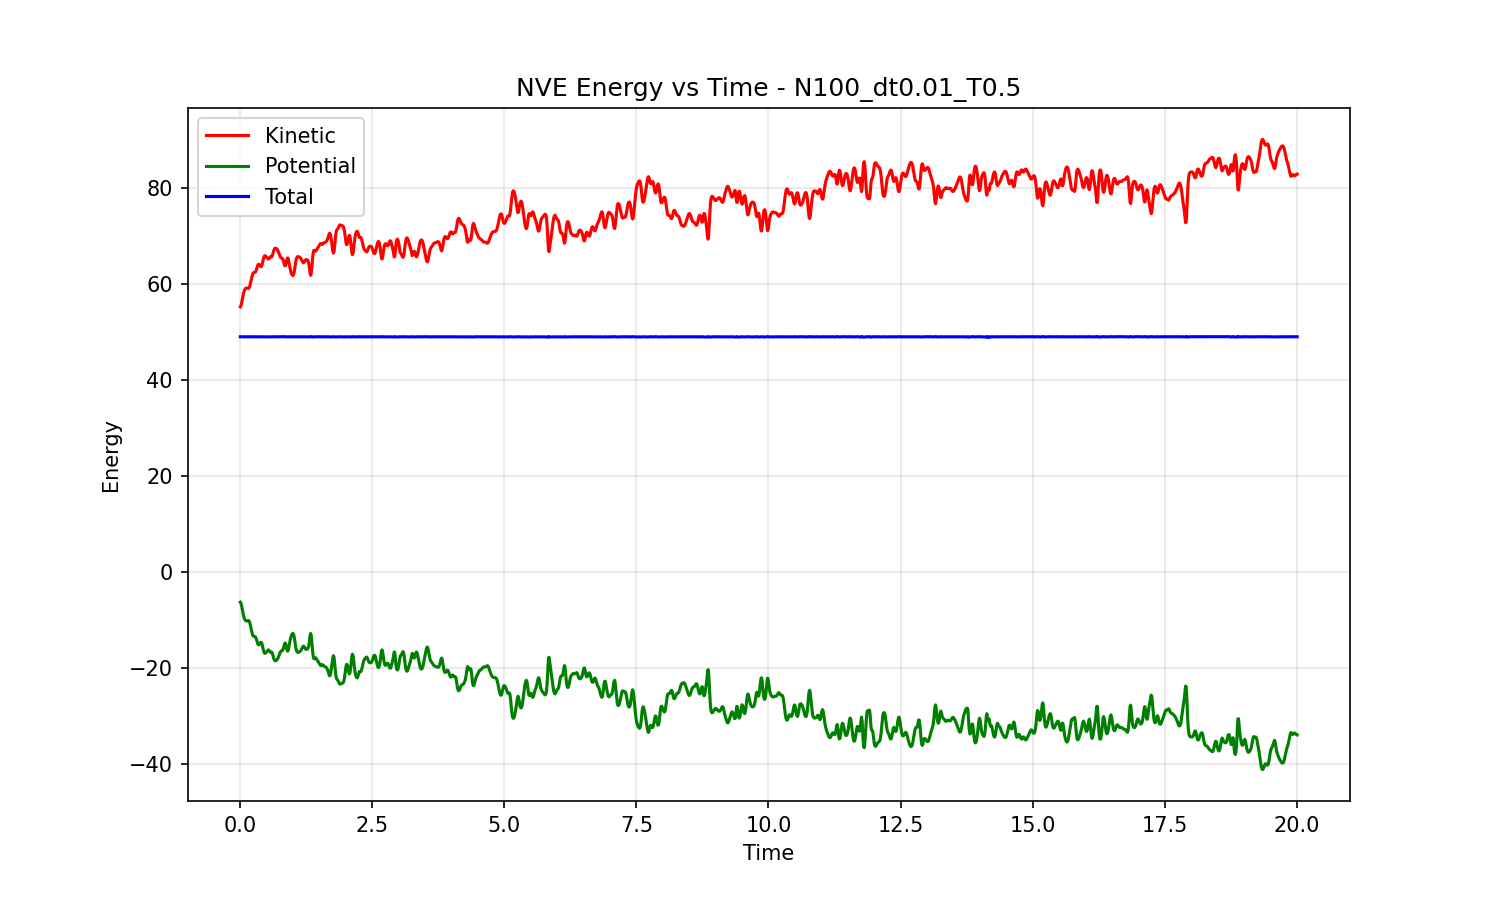
\includegraphics[width=\textwidth]{media/energy_N100_dt0.01_T0.5.png}
		\caption{N=100 particles with dt=0.01 and T=0.5}
		\label{sfig:energy_N100}
	\end{subfigure}%
	~
	\begin{subfigure}{0.5\textwidth}
		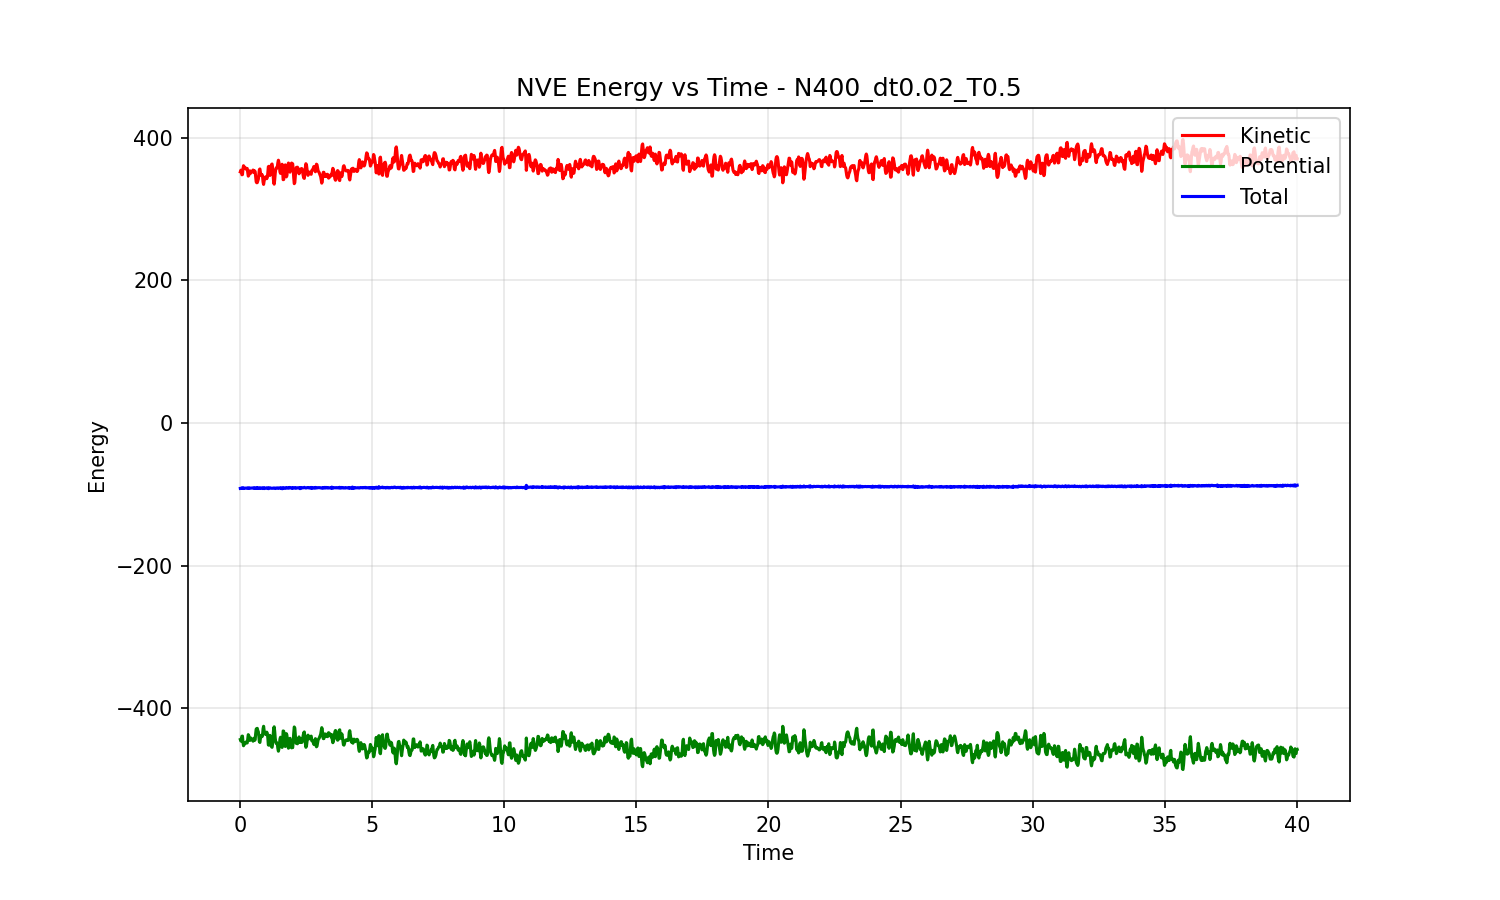
\includegraphics[width=\textwidth]{media/energy_N400_dt0.02_T0.5.png}
		\caption{N=400 particles with dt=0.02 and T=0.5}
		\label{sfig:energy_N400_dt002}
	\end{subfigure}%
	\\
	\begin{subfigure}{0.5\textwidth}
		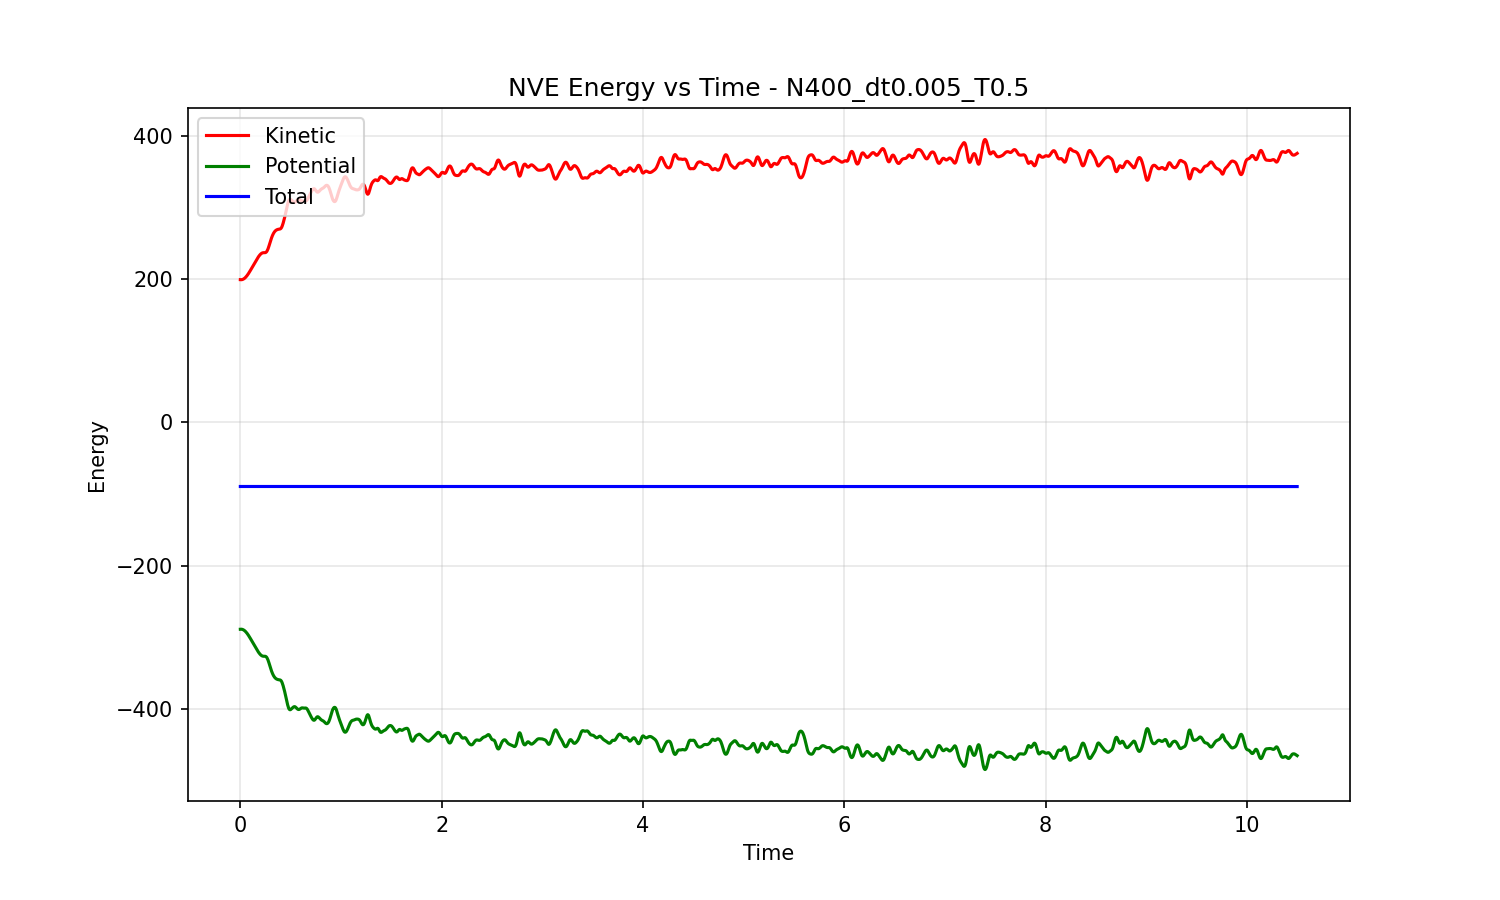
\includegraphics[width=\textwidth]{media/energy_N400_dt0.005_T0.5.png}
		\caption{N=400 particles with dt=0.005 and T=0.5}
		\label{sfig:energy_N400_dt0005}
	\end{subfigure}%
	~
	\begin{subfigure}{0.5\textwidth}
		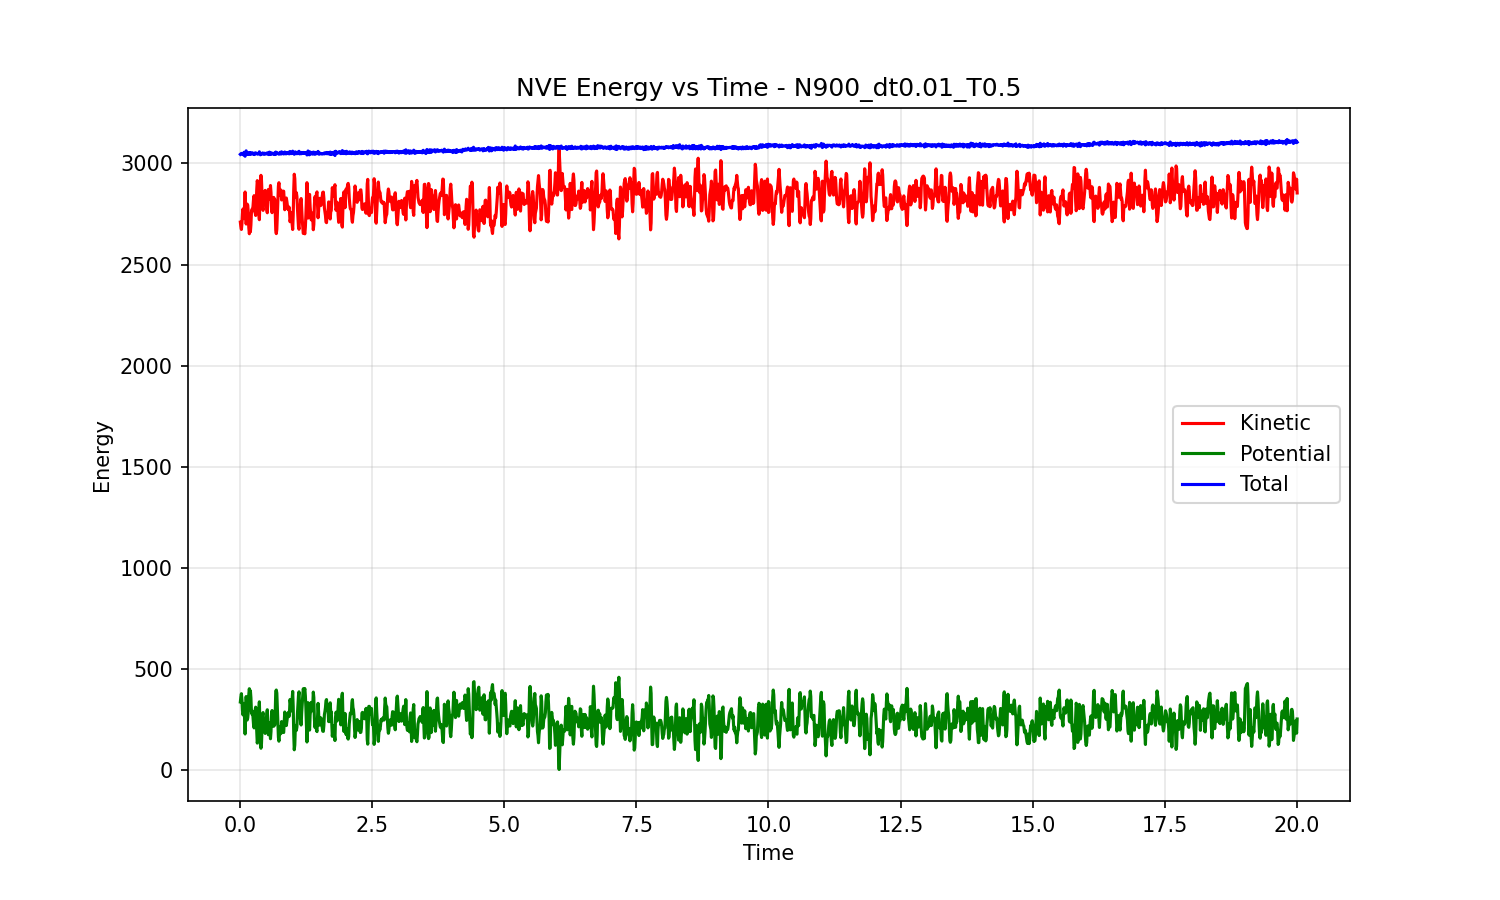
\includegraphics[width=\textwidth]{media/energy_N900_dt0.01_T0.5.png}
		\caption{N=900 particles with dt=0.01 and T=0.5}
		\label{sfig:energy_N900}
	\end{subfigure}%
	\caption{\textbf{Energy Conservation in NVE Ensemble} 
    Analysis of total, kinetic, and potential energies over time for different system configurations.}
	\label{fig:energy_conservation}
\end{figure}
\begin{figure}[H]
	\centering
	\begin{subfigure}{0.5\textwidth}
		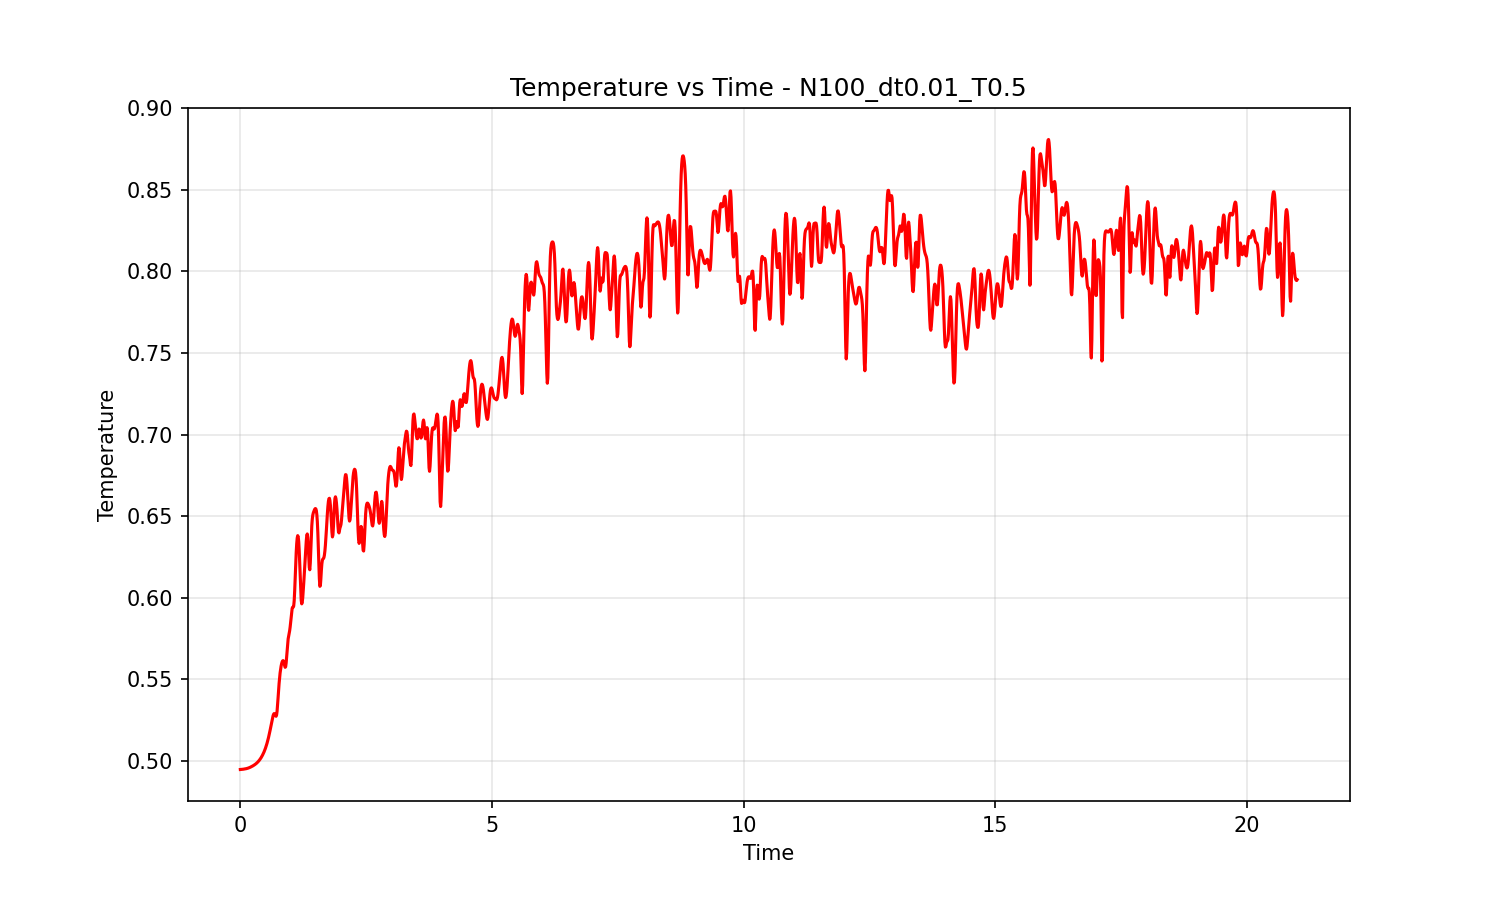
\includegraphics[width=\textwidth]{media/temp_N100_dt0.01_T0.5.png}
		\caption{N=100 particles with dt=0.01 and T=0.5}
		\label{sfig:temp_N100}
	\end{subfigure}%
	~
	\begin{subfigure}{0.5\textwidth}
		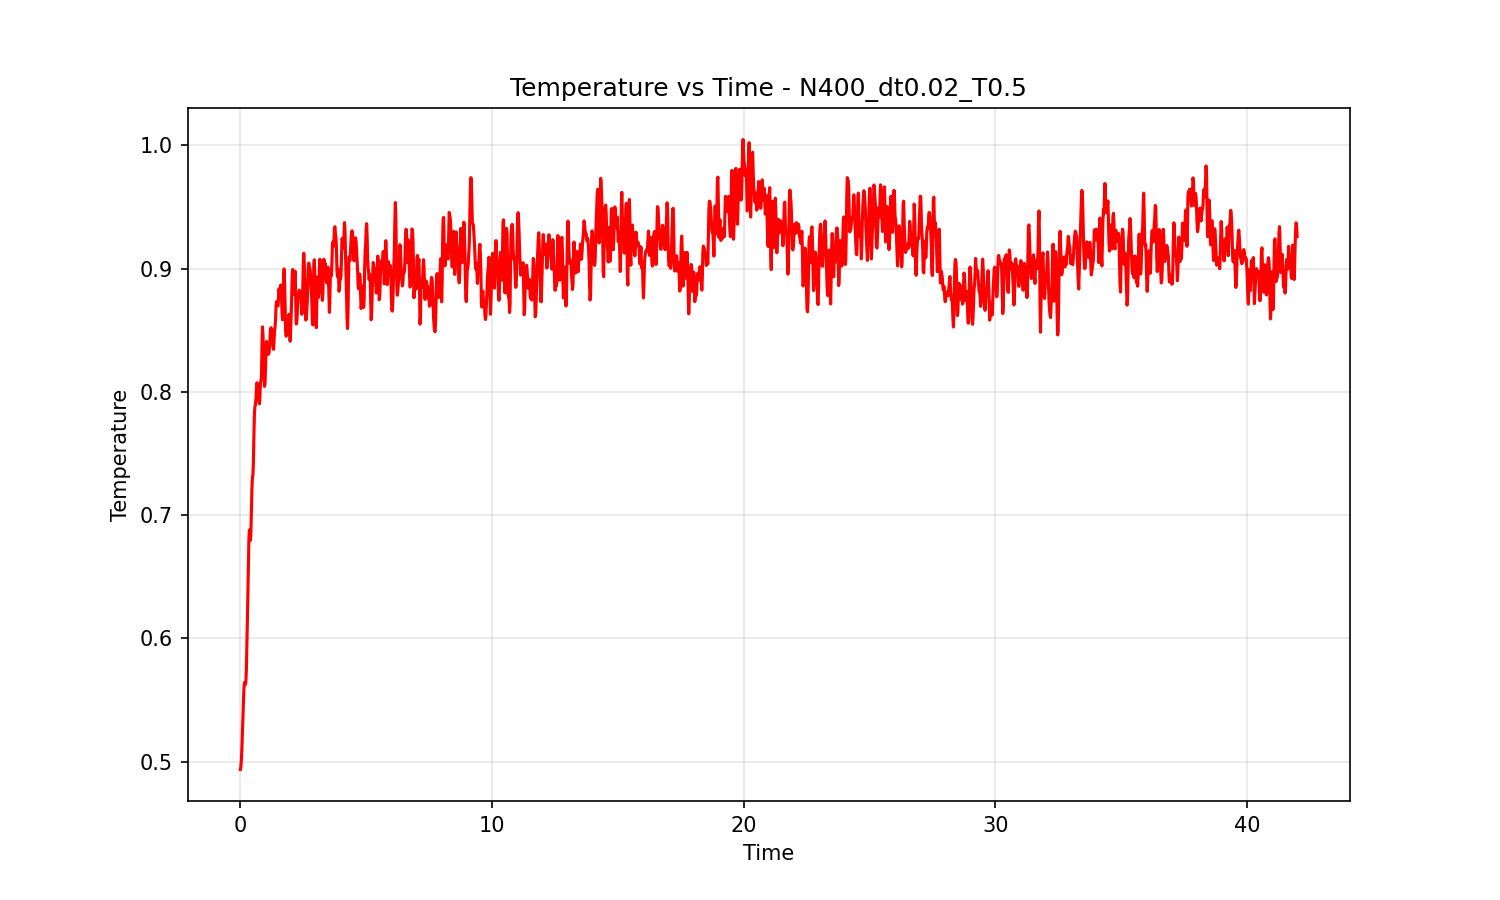
\includegraphics[width=\textwidth]{media/temp_N400_dt0.02_T0.5.png}
		\caption{N=400 particles with dt=0.02 and T=0.5}
		\label{sfig:temp_N400_dt002}
	\end{subfigure}%
	\\
	\begin{subfigure}{0.5\textwidth}
		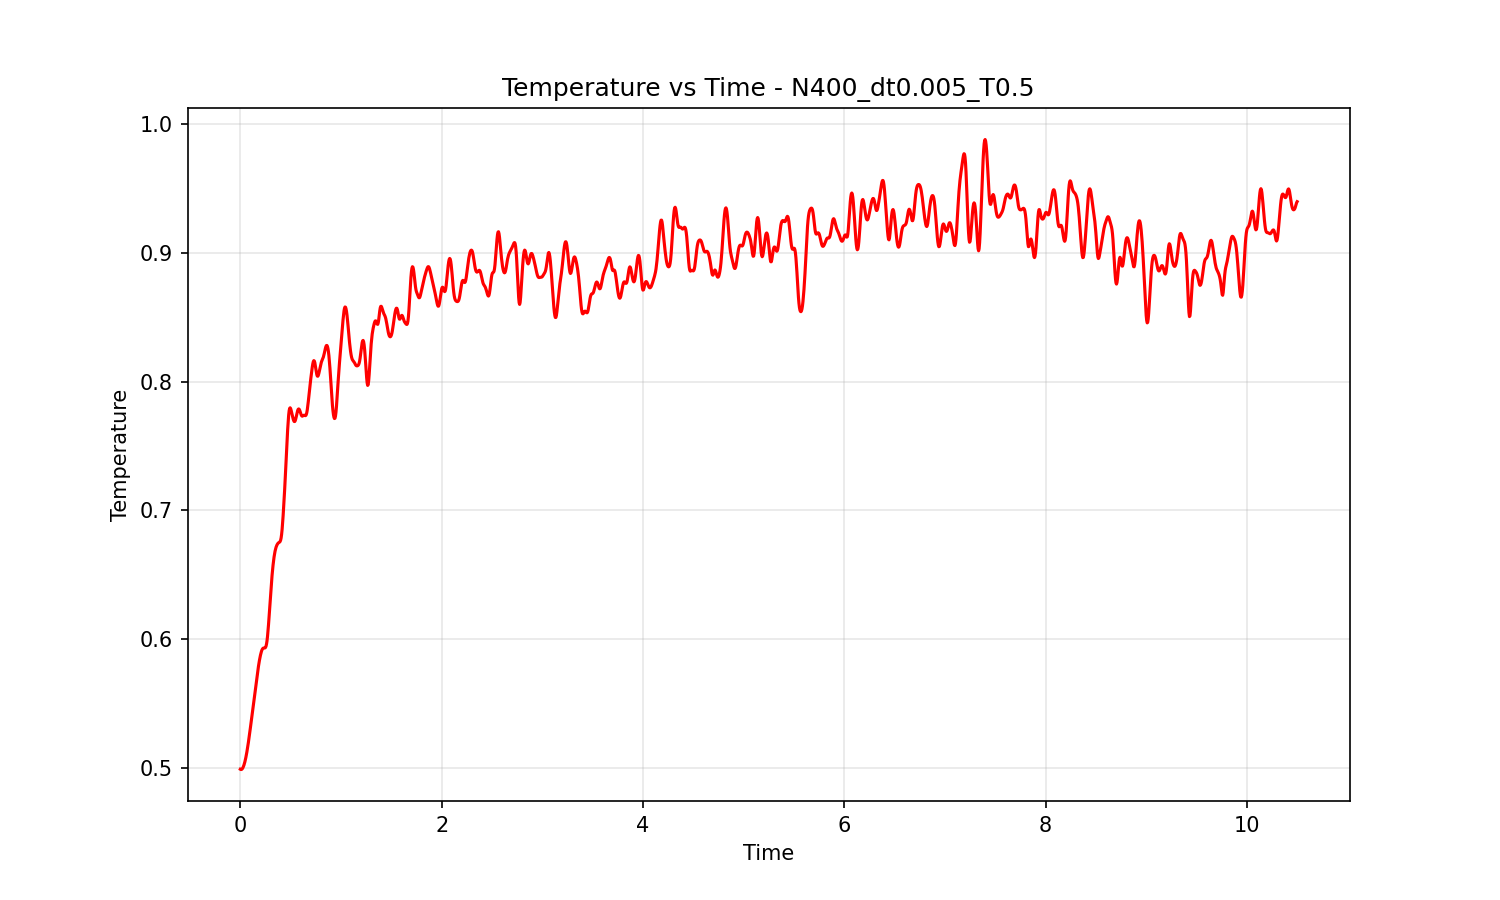
\includegraphics[width=\textwidth]{media/temp_N400_dt0.005_T0.5.png}
		\caption{N=400 particles with dt=0.005 and T=0.5}
		\label{sfig:temp_N400_dt0005}
	\end{subfigure}%
	~
	\begin{subfigure}{0.5\textwidth}
		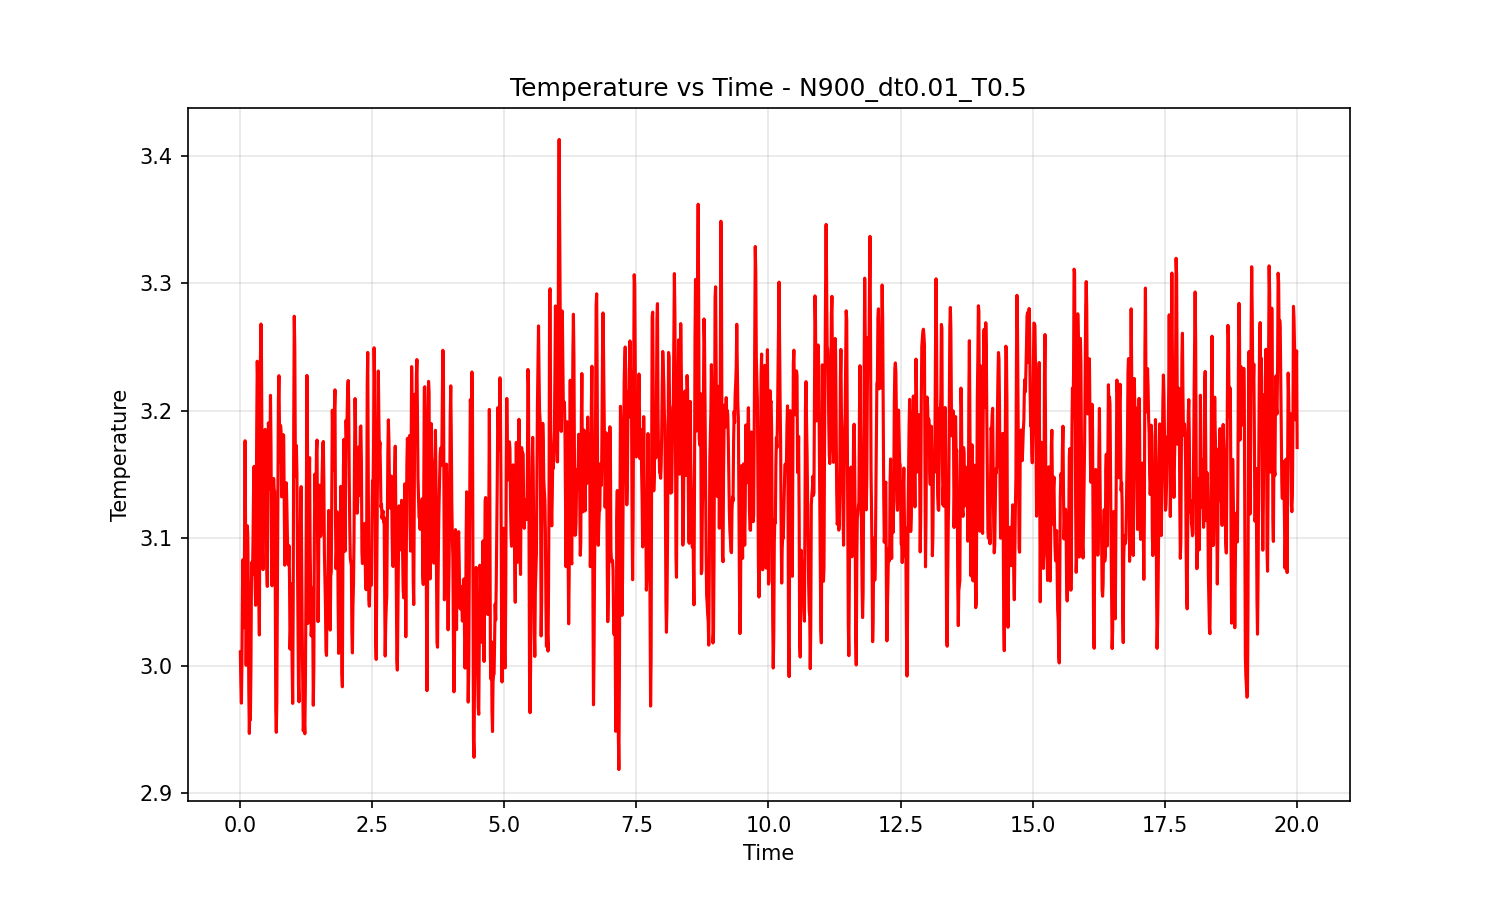
\includegraphics[width=\textwidth]{media/temp_N900_dt0.01_T0.5.png}
		\caption{N=900 particles with dt=0.01 and T=0.5}
		\label{sfig:temp_N900}
	\end{subfigure}%


	\caption{\textbf{Temperature Evolution in NVE Ensemble} 
	Analysis of temperature fluctuations over time for different system configurations.}
	\label{fig:temperature_evolution}
\end{figure}
% \begin{figure}[H]
% 	\centering
% 	\begin{subfigure}{0.5\textwidth}
% 		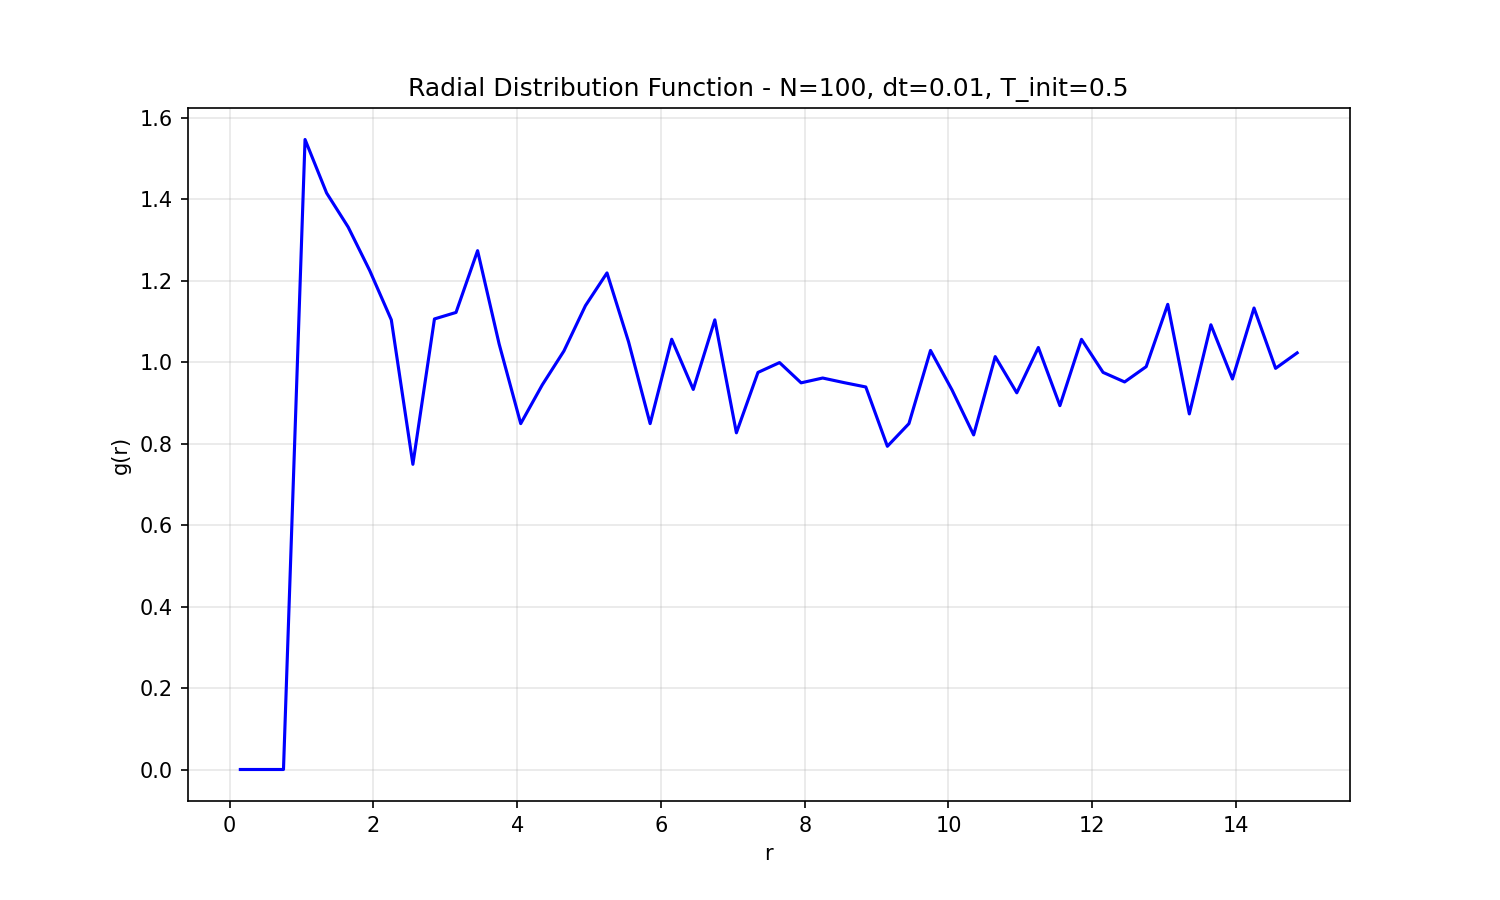
\includegraphics[width=\textwidth]{media/final_rdf_N100_dt0.01_T0.5_final.png}
% 		\caption{N=100 particles with dt=0.01 and T=0.5}
% 		\label{sfig:rdf_N100}
% 	\end{subfigure}%
% 	~
% 	\begin{subfigure}{0.5\textwidth}
% 		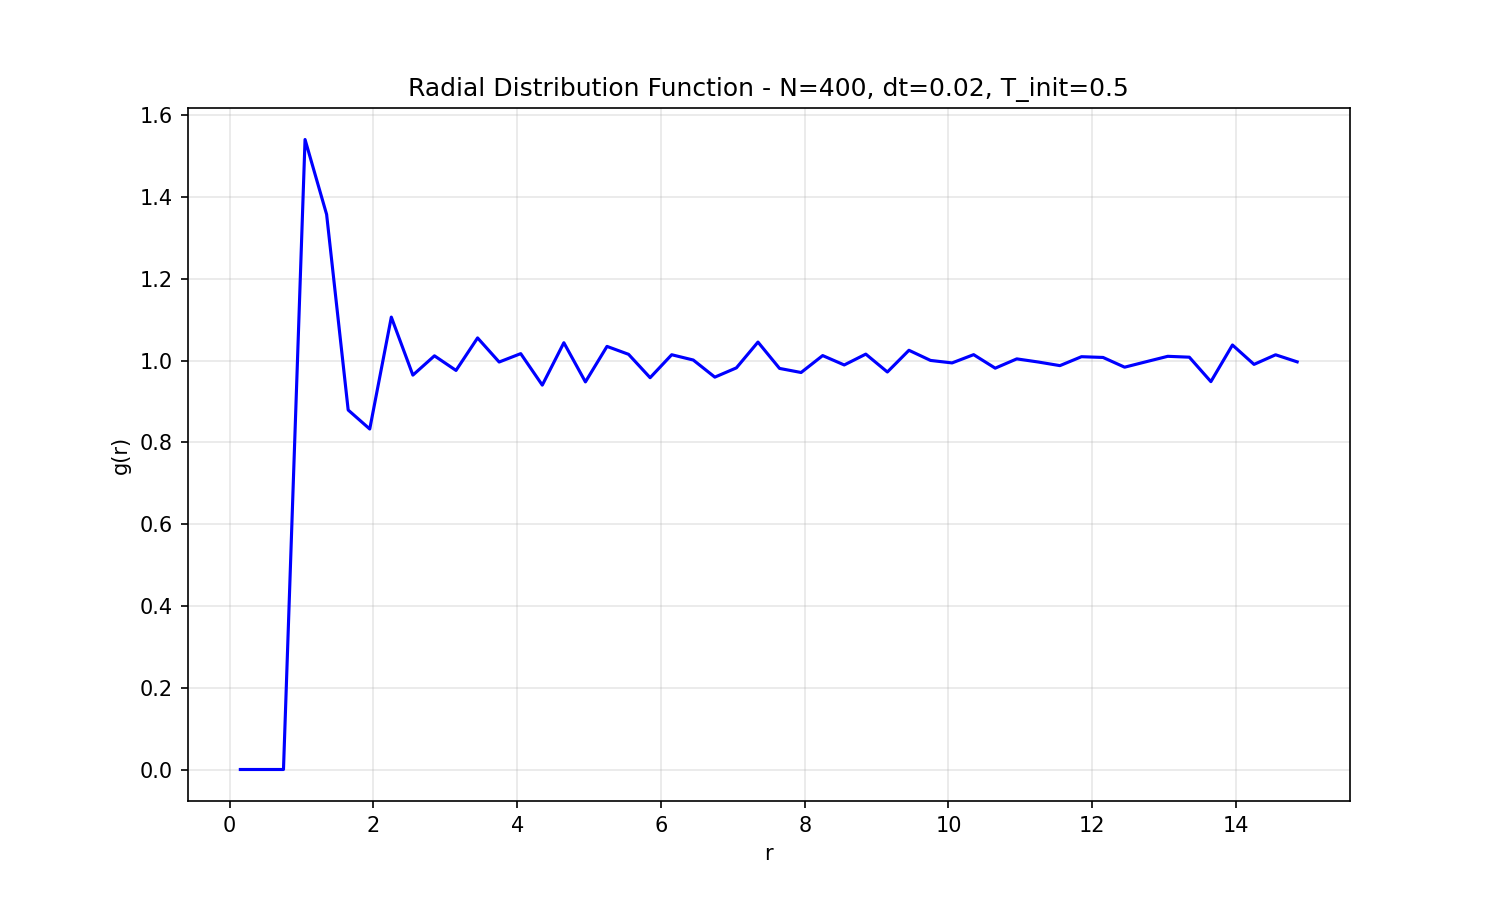
\includegraphics[width=\textwidth]{media/final_rdf_N400_dt0.02_T0.5_final.png}
% 		\caption{N=400 particles with dt=0.02 and T=0.5}
% 		\label{sfig:rdf_N400_dt002}
% 	\end{subfigure}%
% 	\\
% \begin{subfigure}{0.5\textwidth}
% 		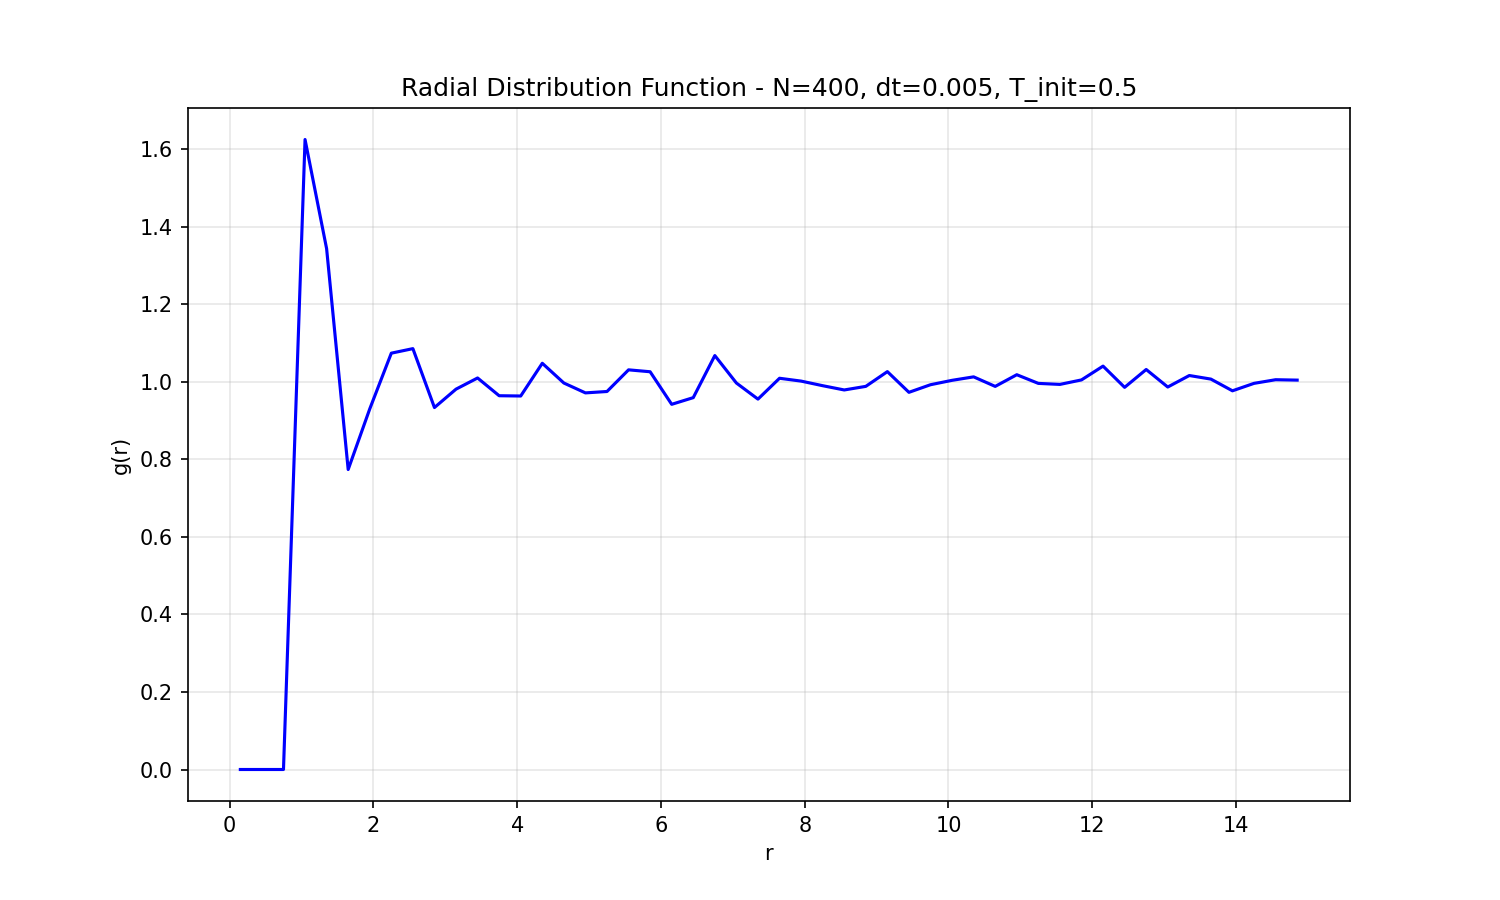
\includegraphics[width=\textwidth]{media/final_rdf_N400_dt0.005_T0.5_final.png}
% 		\caption{N=400 particles with dt=0.005 and T=0.5}
% 		\label{sfig:rdf_N400_dt0005}
% 	\end{subfigure}%
% 	~
% 	\begin{subfigure}{0.5\textwidth}
% 		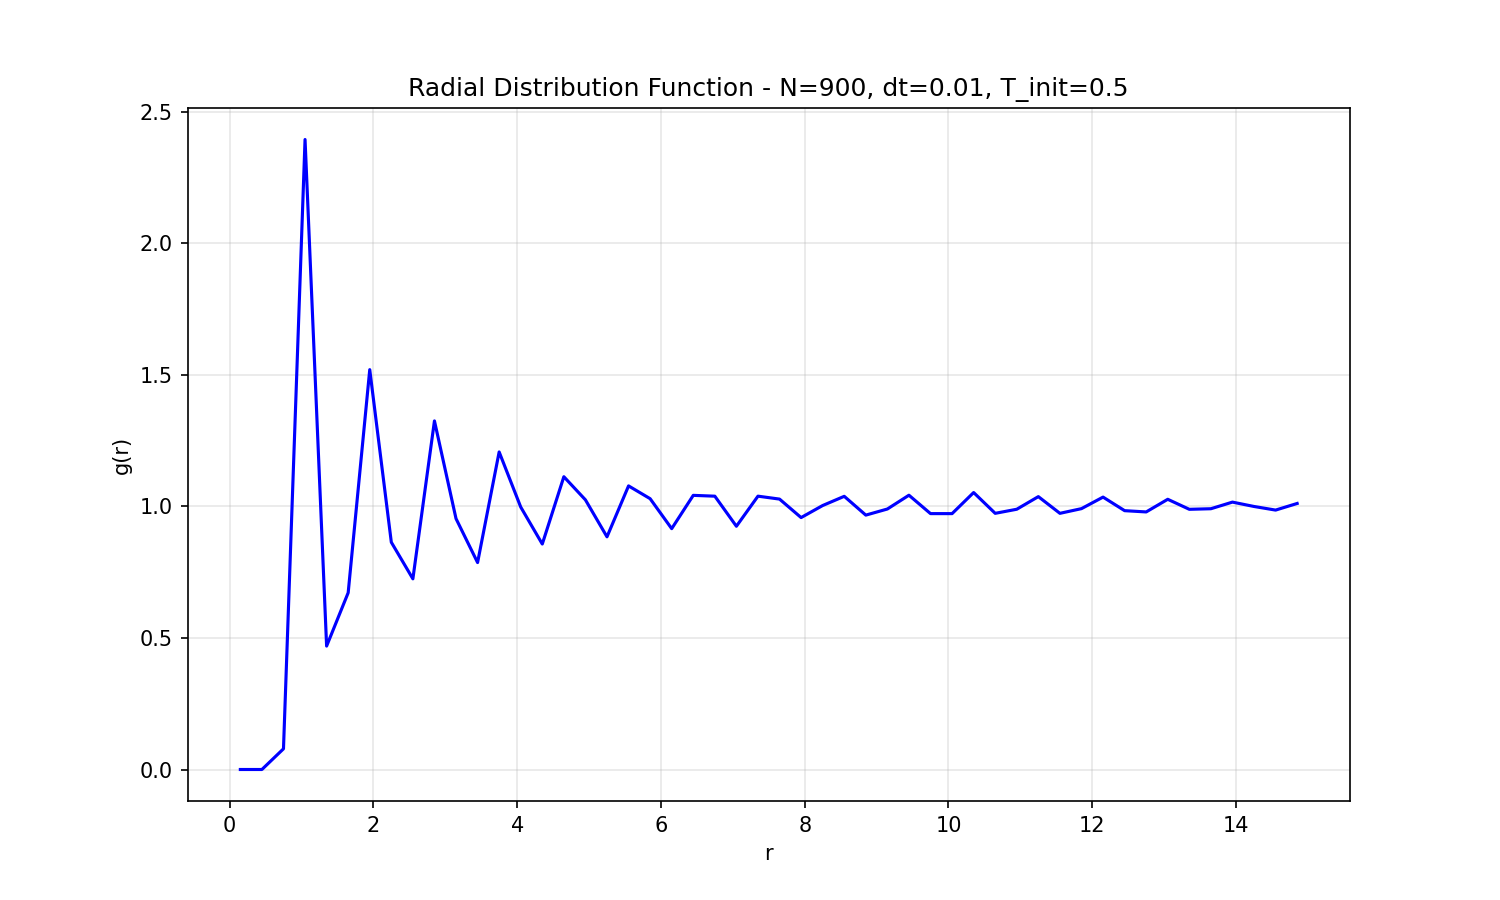
\includegraphics[width=\textwidth]{media/final_rdf_N900_dt0.01_T0.5_final.png}
% 		\caption{N=900 particles with dt=0.01 and T=0.5}
% 		\label{sfig:rdf_N900}
% 	\end{subfigure}%
% 	\caption{\textbf{Radial Distribution Functions (RDF) in NVE Ensemble} 
% 	Final radial distribution functions for different system configurations.}
% 	\label{fig:radial_distribution}
% \end{figure}
\begin{figure}[H]
	\centering
	\begin{subfigure}{0.5\textwidth}
		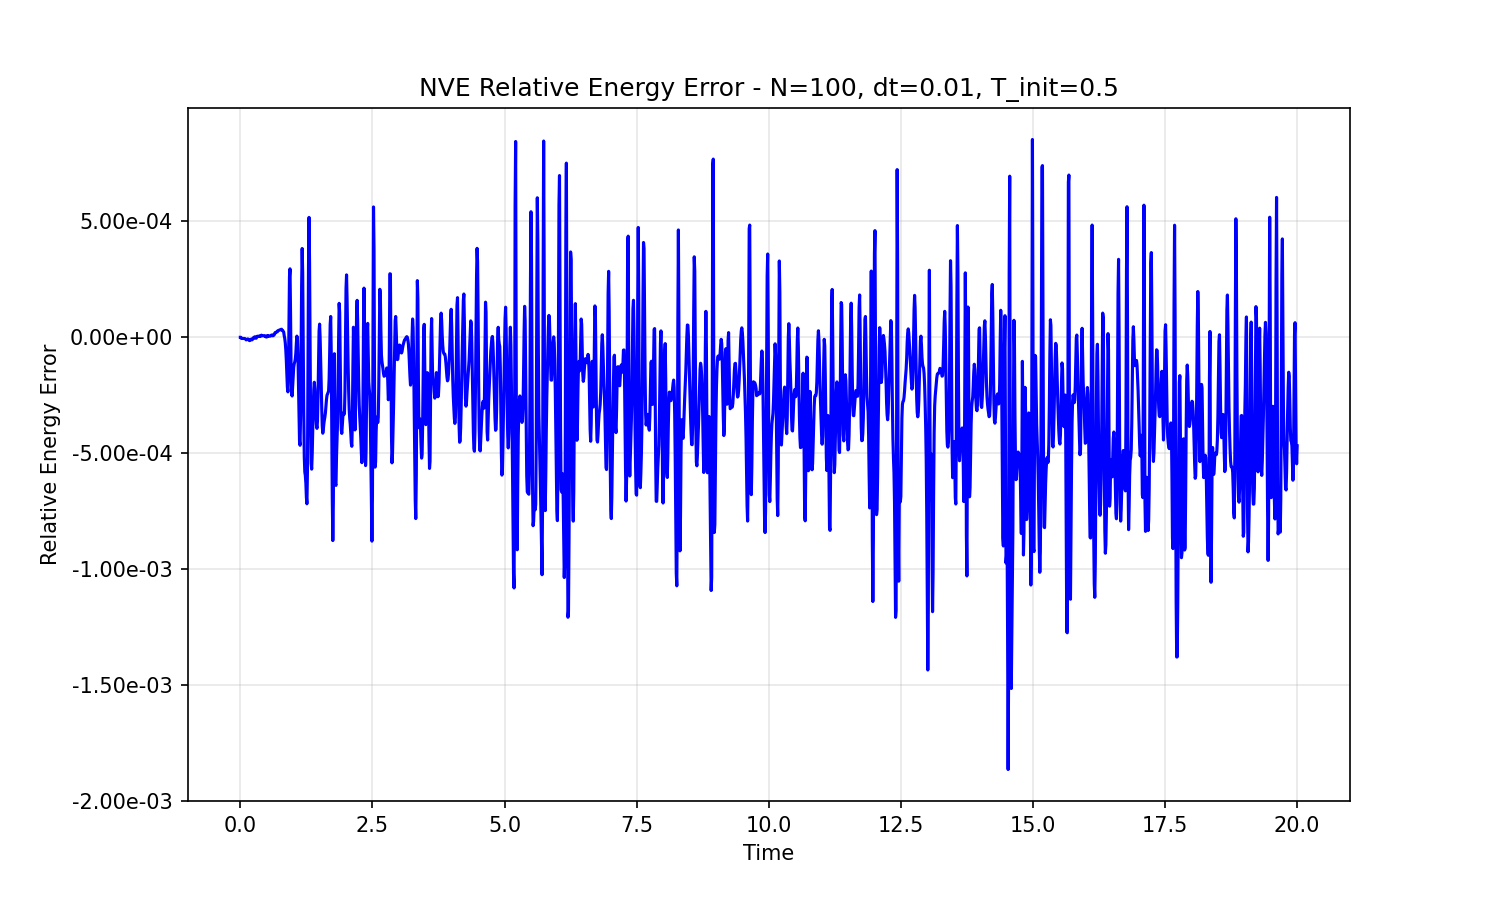
\includegraphics[width=\textwidth]{media/error_N100_dt0.01_T0.5.png}
		\caption{N=100 particles with dt=0.01 and T=0.5}
		\label{sfig:error_N100}
	\end{subfigure}%
	~
	\begin{subfigure}{0.5\textwidth}
		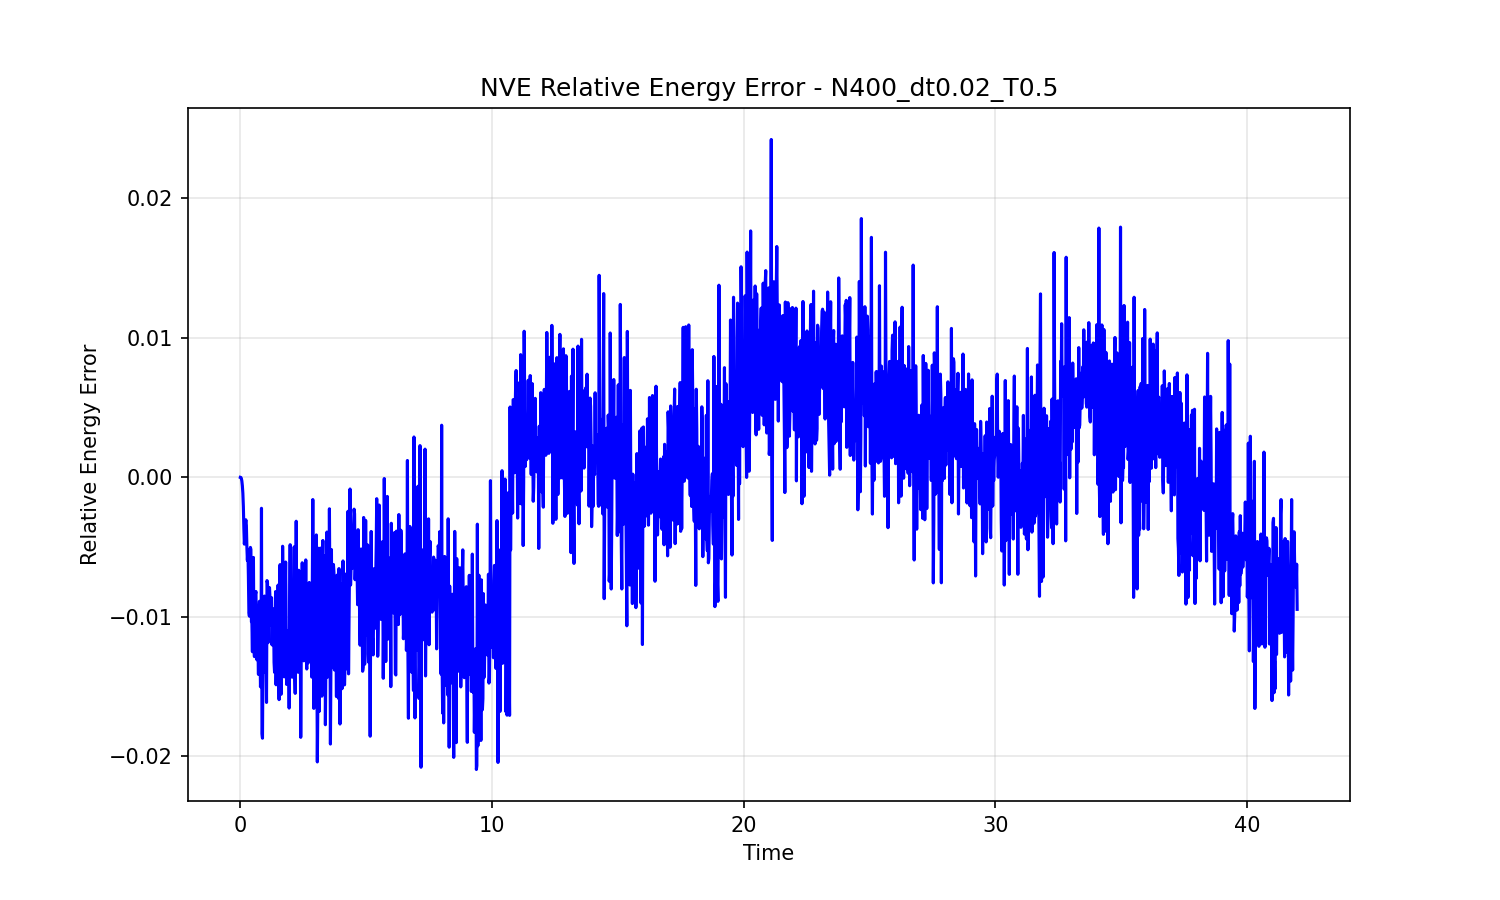
\includegraphics[width=\textwidth]{media/error_N400_dt0.02_T0.5.png}
		\caption{N=400 particles with dt=0.02 and T=0.5}
		\label{sfig:error_N400_dt002}
	\end{subfigure}%
	\\
	\begin{subfigure}{0.5\textwidth}
		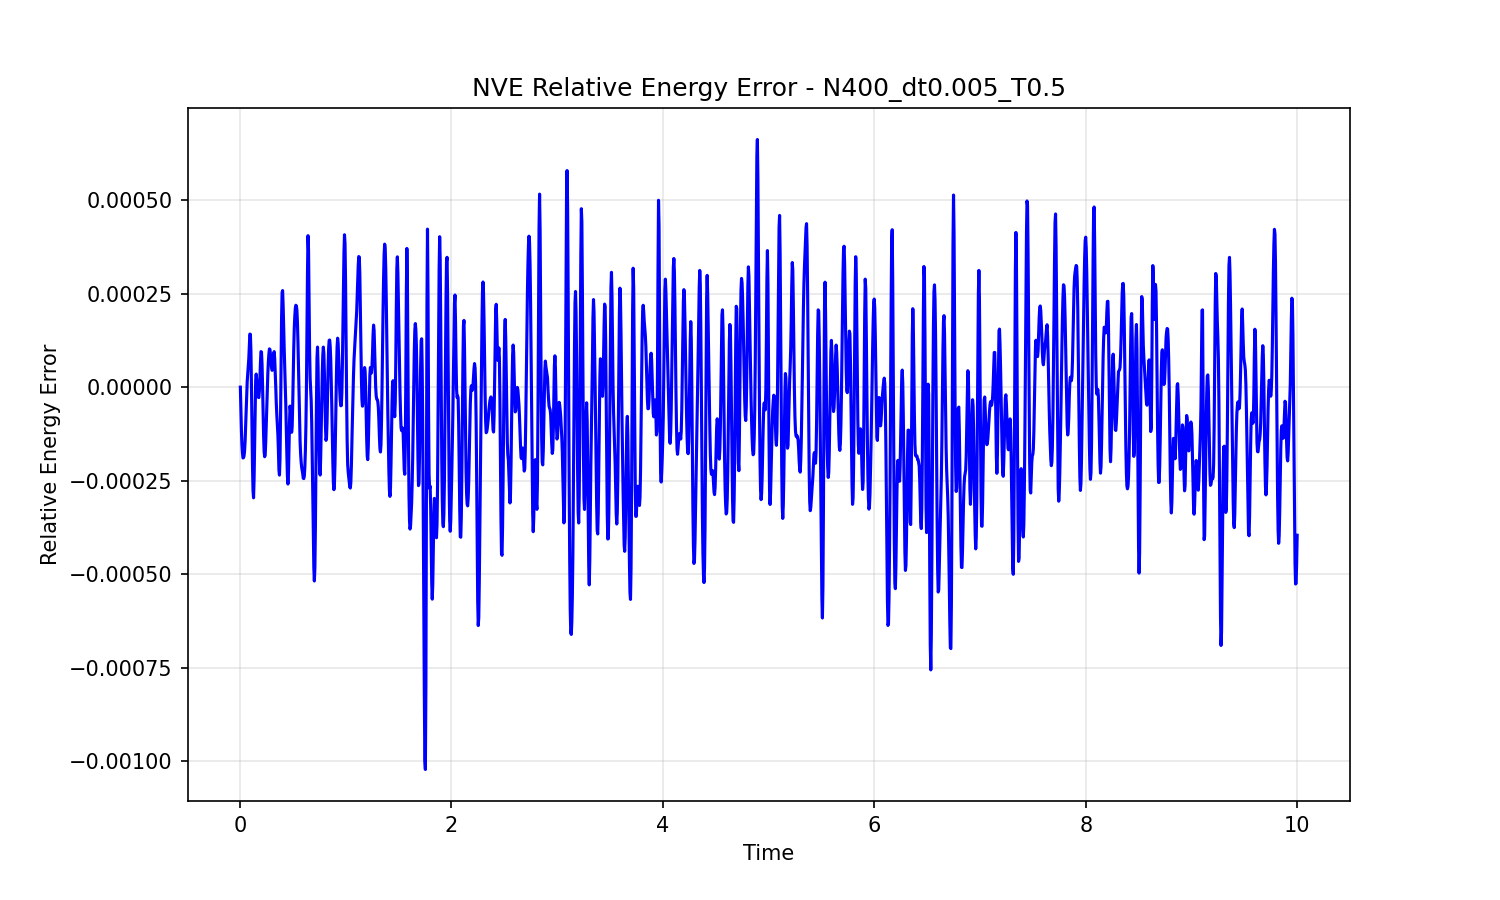
\includegraphics[width=\textwidth]{media/error_N400_dt0.005_T0.5.png}
		\caption{N=400 particles with dt=0.005 and T=0.5}
		\label{sfig:error_N400_dt0005}
	\end{subfigure}%
	~
\begin{subfigure}{0.5\textwidth}
		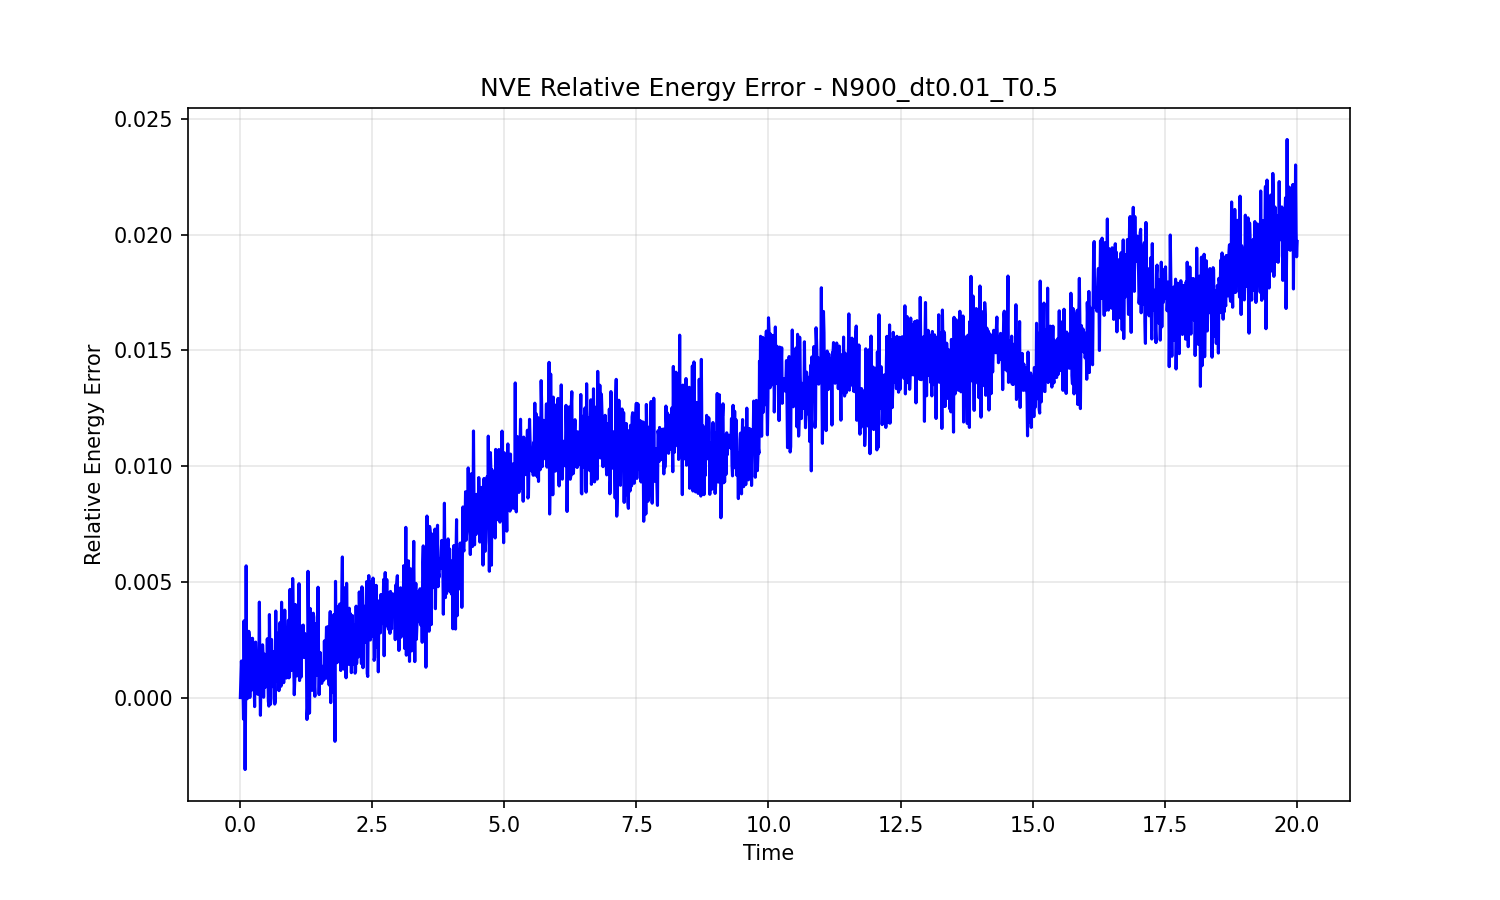
\includegraphics[width=\textwidth]{media/error_N900_dt0.01_T0.5.png}
		\caption{N=900 particles with dt=0.01 and T=0.5}
		\label{sfig:error_N900}
	\end{subfigure}%

	\caption{\textbf{Energy Conservation Error Analysis in NVE Ensemble} 
	Relative energy conservation error over time for different system configurations.}
	\label{fig:energy_error}
\end{figure}
% section Energy-Conserving Dynamics: The NVE Ensemble (end)

\section{Temperature-Regulated Dynamics: The NVT Ensemble}
% The canonical ensemble (NVT), on the other hand, maintains constant number of particles (N), volume (V), and temperature (T) through the use of a thermostat—in our case, the Berendsen thermostat.
For the NVT simulation we use the Berendsen thermostat with a relaxation time parameter of $\frac{dt}{\tau} = 0.0025$ to maintain constant temperature using various number of particles and target temperatures. In order to analyze the results we use the temperature evolution plots (Figure~\ref{fig:nvt_temperature}), which show how the system reaches its target temperature. Furthermore we plot the radial distribution function, shown in Figure~\ref{fig:nvt_rdf} at the final time step, showing how density varies as a function of distance.
\subsection{Temperature Regulation}
In Figure~\ref{fig:nvt_temperature} the plot show the application of the Berendsen thermostat across different configurations, the following observation can be made for each individual plot:
\begin{itemize}
	\item For $N=100$ and $T=0.1$ in Subfigure~\ref{sfig:nvt_temp_N100_T01} we observe that the thermostat fails to precisely maintain the target temperature, instead having an equilibrium at roughly $0.12$ with very large oscillations. This shows that the Berendsen thermostat struggles to control the temperature in small systems at low temperatures. This could suggest to adjust the relaxation parameter, so the thermostat can more effectively handle the temperature.
	\item For $N=100$ and $T=1.0$ in Subfigure~\ref{sfig:nvt_temp_N100_T10} the system shows initially temperature higher than the target temperature and then afterwards it approaches the target temperature and starts oscillating around it. These oscillations are rather high indicating the challenge of precise temperature control in small systems.
	\item For $N=625$ and $T=1.0$ in Subfigure~\ref{sfig:nvt_temp_N625_T10} similar to the previous case we can observe a similar pattern of initial equilibration phase and then an oscillation around the target temperature, but in this case the system has reduced fluctuations amplitudes. This indicates that an increasing number of particles improves the temperature stability.
	\item For $N=900$ and $T=1.0$ in Subfigure~\ref{sfig:nvt_temp_N900_T10} we can observe that the system starts at a significantly higher temperature than the target temperature and then gradually decreases until it reaches the target temperature. In comparison to the other cases this cooling process is rather smooth, which highlights the stability of system with a higher number of particles.
\end{itemize}
\begin{figure}[H]
	\centering
	\begin{subfigure}{0.5\textwidth}
		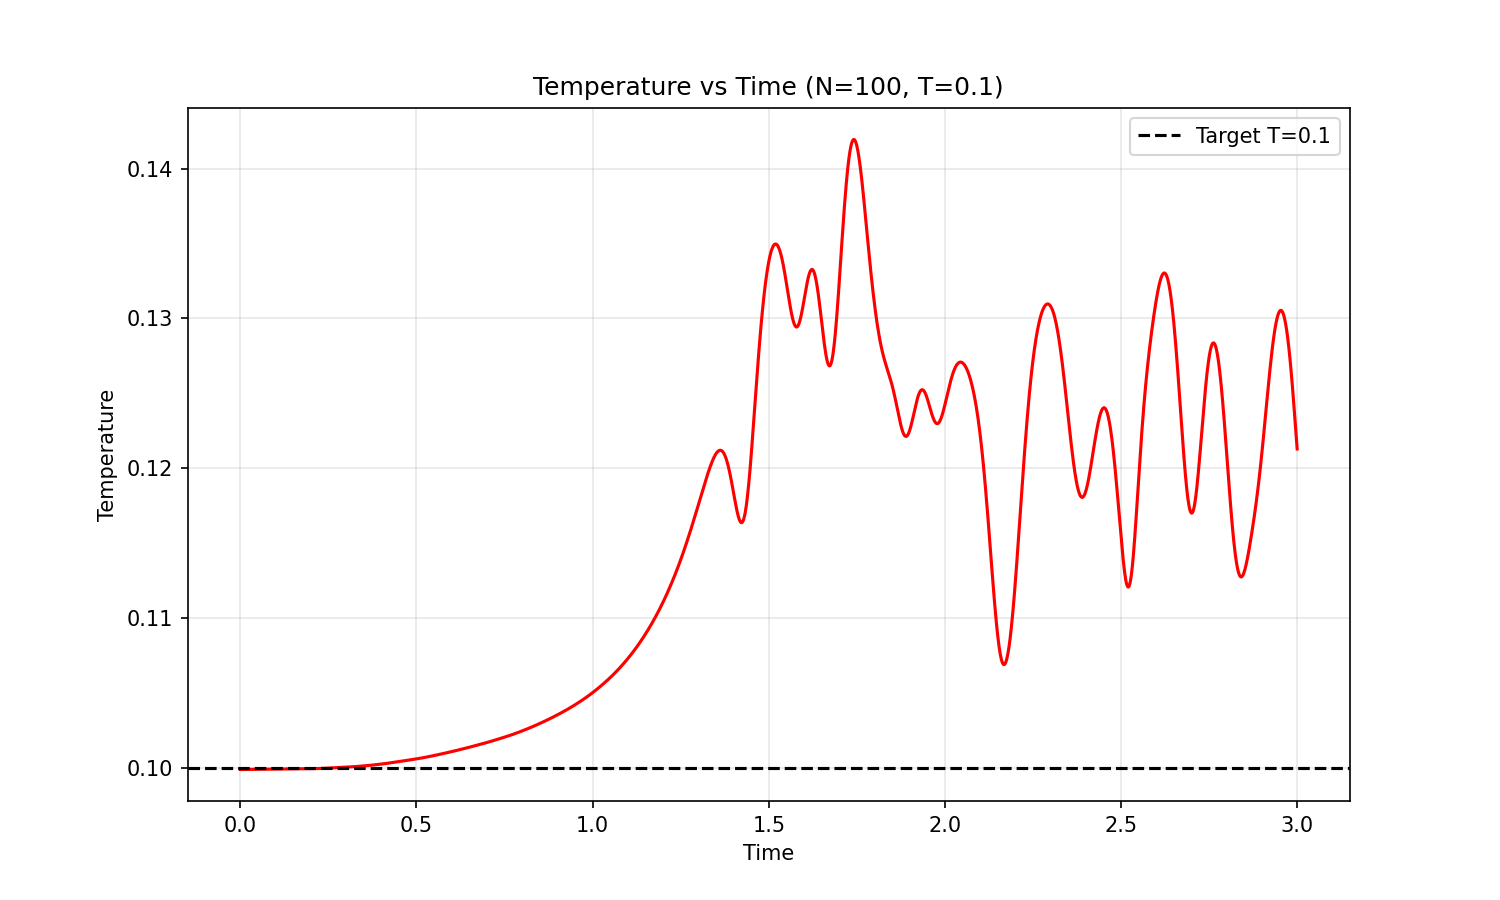
\includegraphics[width=\textwidth]{media/temp_N100_T0.1.png}
		\caption{N=100 particles with T=0.1}
		\label{sfig:nvt_temp_N100_T01}
	\end{subfigure}%
	~
	\begin{subfigure}{0.5\textwidth}
		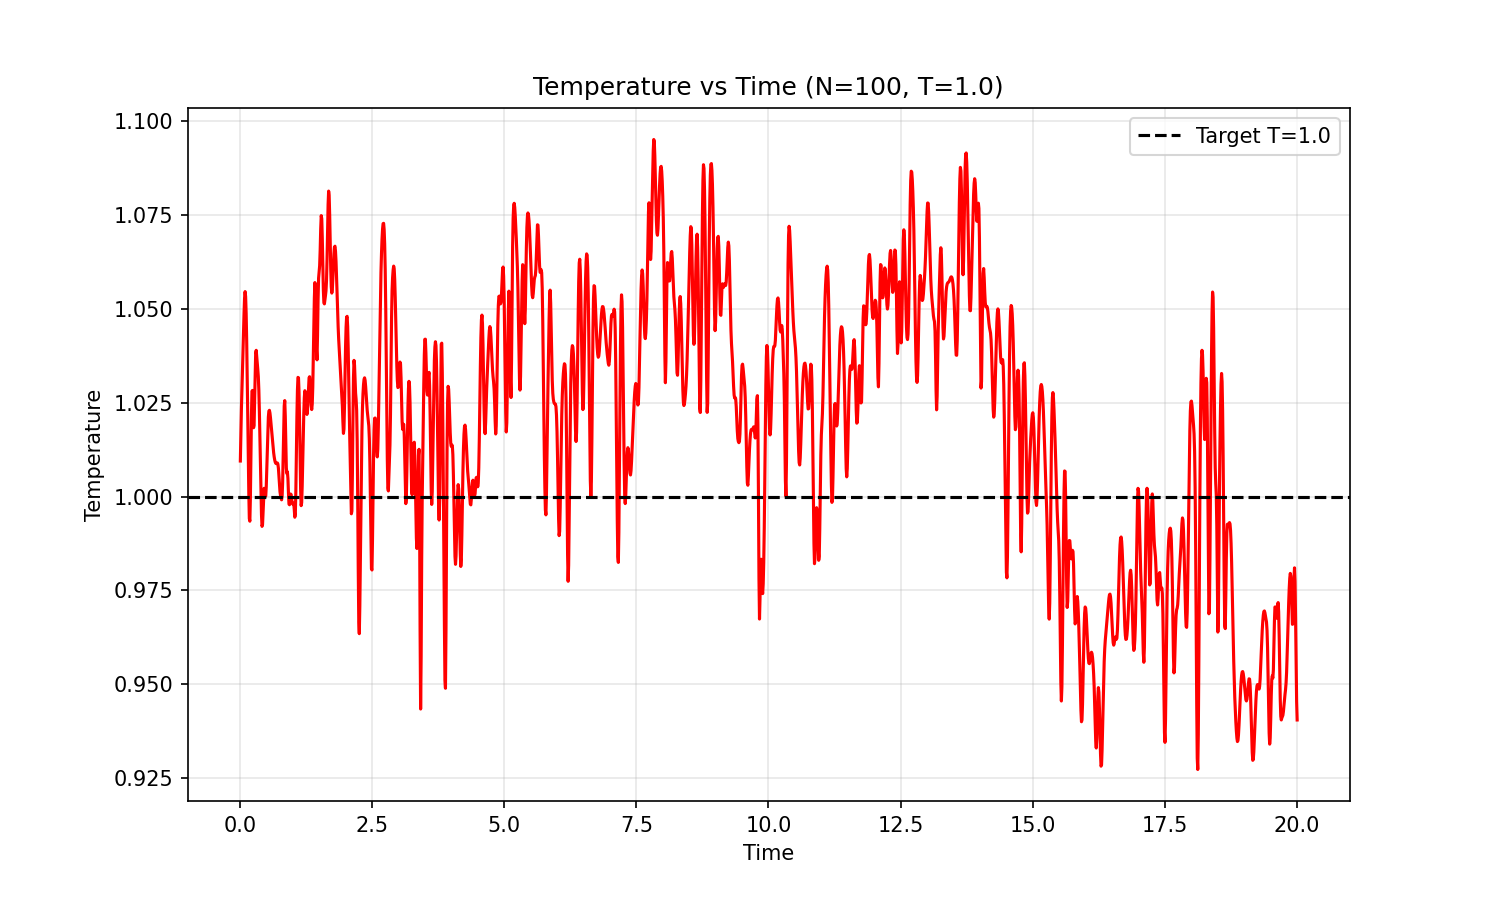
\includegraphics[width=\textwidth]{media/temp_N100_T1.0.png}
		\caption{N=100 particles with T=1.0}
		\label{sfig:nvt_temp_N100_T10}
	\end{subfigure}%
	\\
	\begin{subfigure}{0.5\textwidth}
		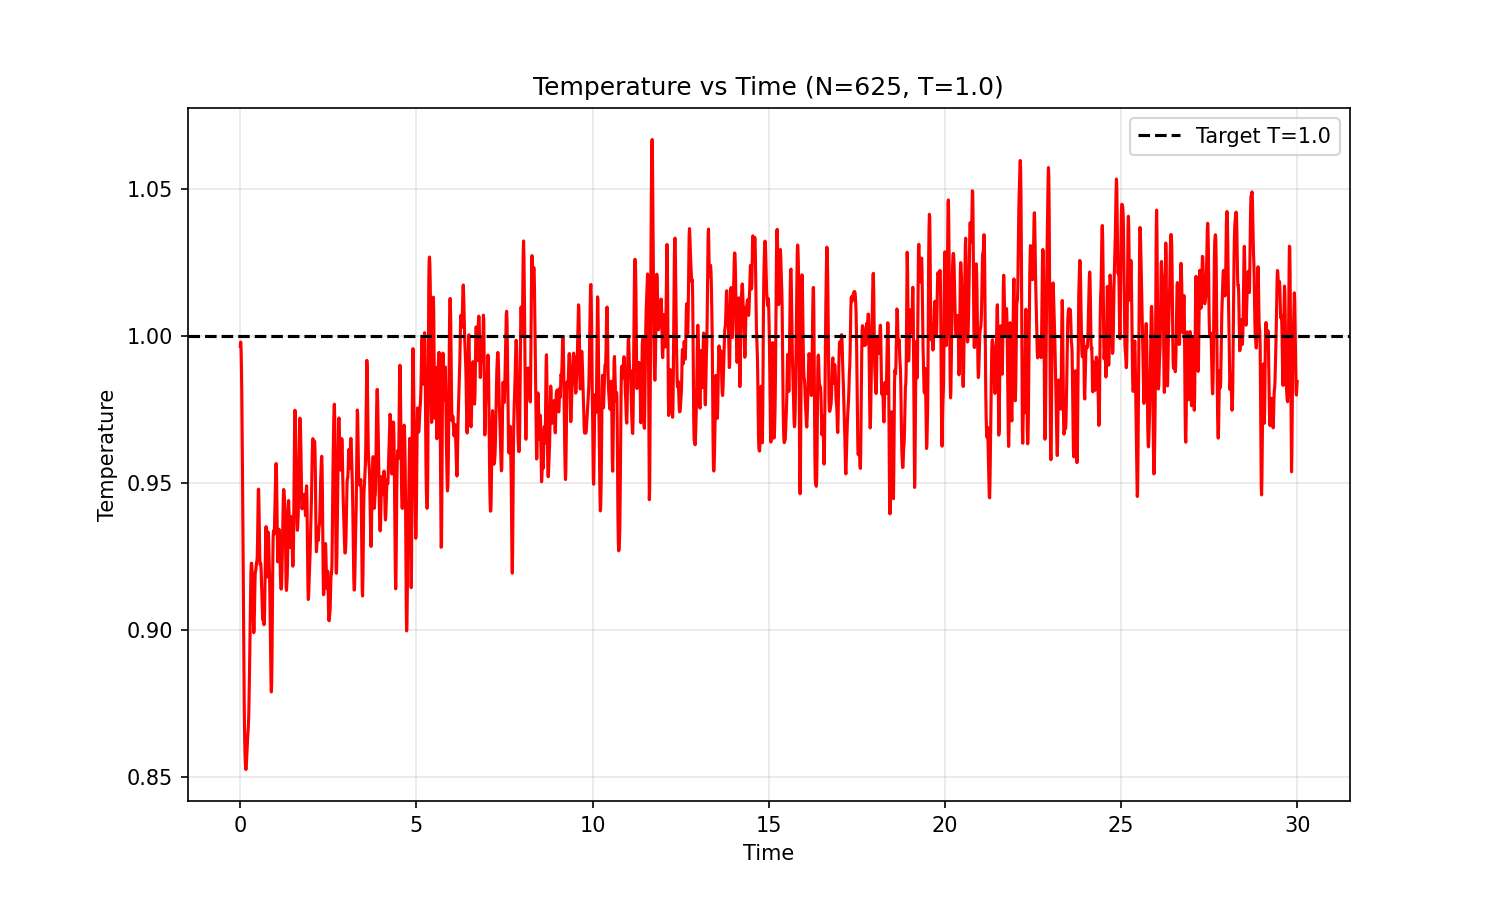
\includegraphics[width=\textwidth]{media/temp_N625_T1.0.png}
		\caption{N=625 particles with T=1.0}
		\label{sfig:nvt_temp_N625_T10}
	\end{subfigure}%
	~
	\begin{subfigure}{0.5\textwidth}
		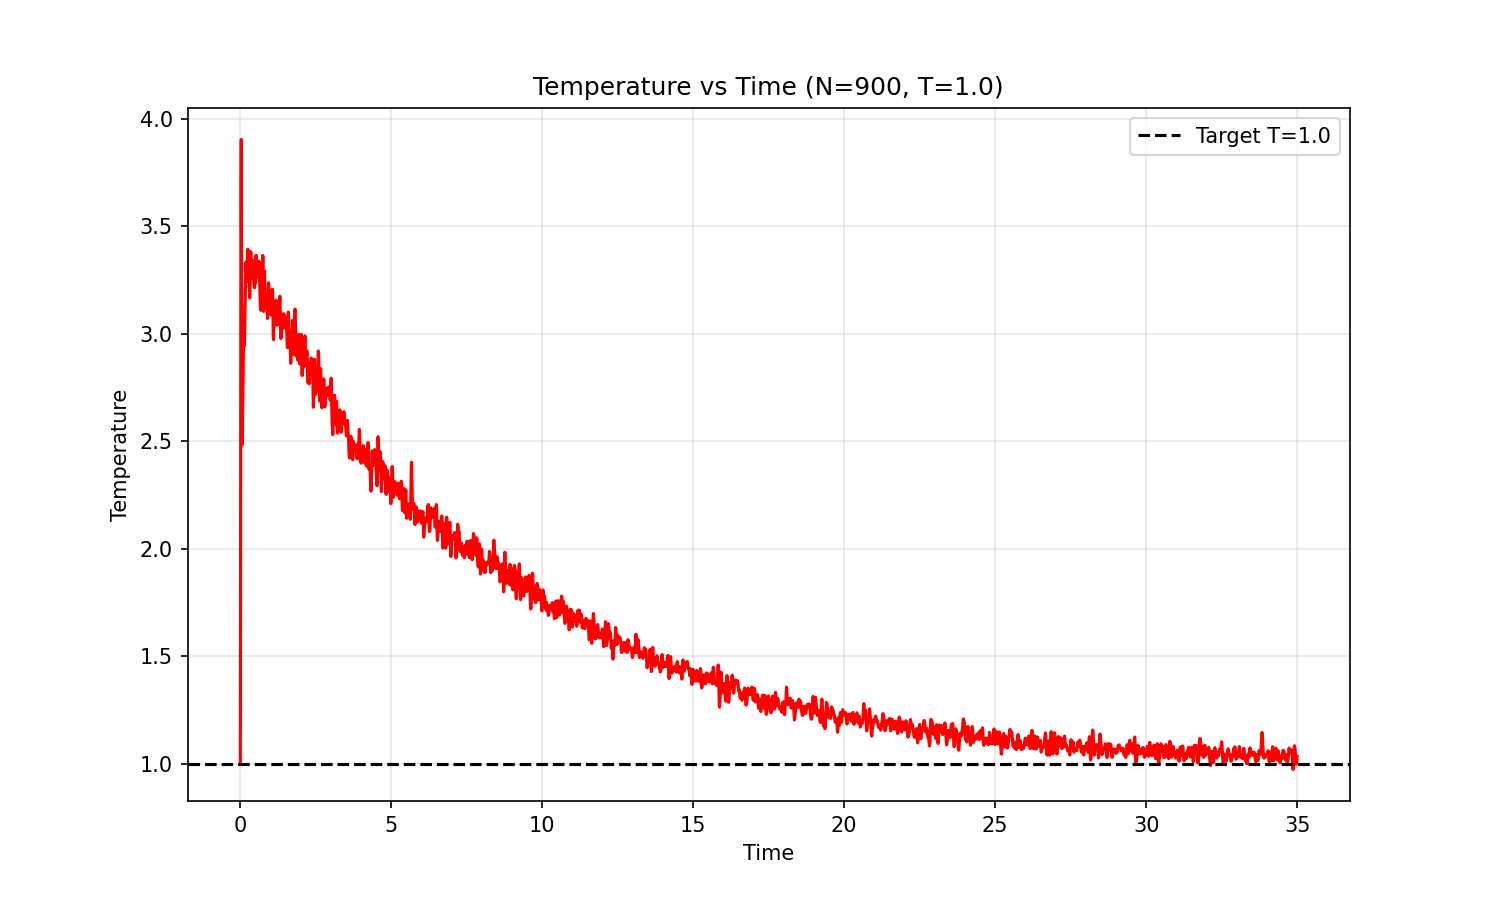
\includegraphics[width=\textwidth]{media/temp_N900_T1.0.png}
		\caption{N=900 particles with T=1.0}
		\label{sfig:nvt_temp_N900_T10}
	\end{subfigure}%
	\caption{\textbf{Temperature Regulation in NVT Ensemble}
		Temperature evolution for different system configurations using the Berendsen thermostat.}
	\label{fig:nvt_temperature}
\end{figure}
\subsection{Radial Distribution Analysis}
Figure~\ref{fig:nvt_rdf} shows the radial distribution function, after equilibration for each of the system configurations. This reveals crucial insight into of the organization of the particles and even allows us to identify the physical state of the matter.
\begin{itemize}
	\item For $N=100$ and $T=0.1$ in Subfigure~\ref{sfig:nvt_rdf_N100_T01} the RDF shows strong oscillations with distinct peaks extending to large distances. This indicates a solid crystalline structure, where the particles maintain a shell like structure of neighbors at specific distances. Due to the low temperature the movement of the particle is severely impaired, resulting in an order structure with long range correlation.
	\item For $N=100$ and $T=1.0$ in Subfigure~\ref{sfig:nvt_rdf_N100_T10} the RDF presents a clear pronounced peak around 1.1, afterwards we can observe less defined peaks. This would indicate either a low-density liquid or possibly a dense gas.
	\item For $N=625$ and $T=1.0$ in Subfigure~\ref{sfig:nvt_rdf_N625_T10} the RDF again shows a clear peak, followed by a smooth approach towards unity at larger distances. This is characteristic behavior for a liquid phase with moderate density.
	\item For $N=900$ and $T=1.0$ in Subfigure~\ref{sfig:nvt_rdf_N900_T10} the RDF exhibits a well defined structure with multiple distinguishable peaks even for large distances. The higher number of particles leads to a high compressed liquid or a dense amorphous state. The system shows enhanced structural organization, due to its high density, placing it closer to liquid-solid phase.
\end{itemize}
Another important observation is the across all the RDFs the first peak occurs around $r=1.1$, which corresponds closely to the expected minimum of the Lennard-Jones Potential, giving further insurance to the validity of the simulations.
\begin{figure}[H]
	\centering
	\begin{subfigure}{0.5\textwidth}
		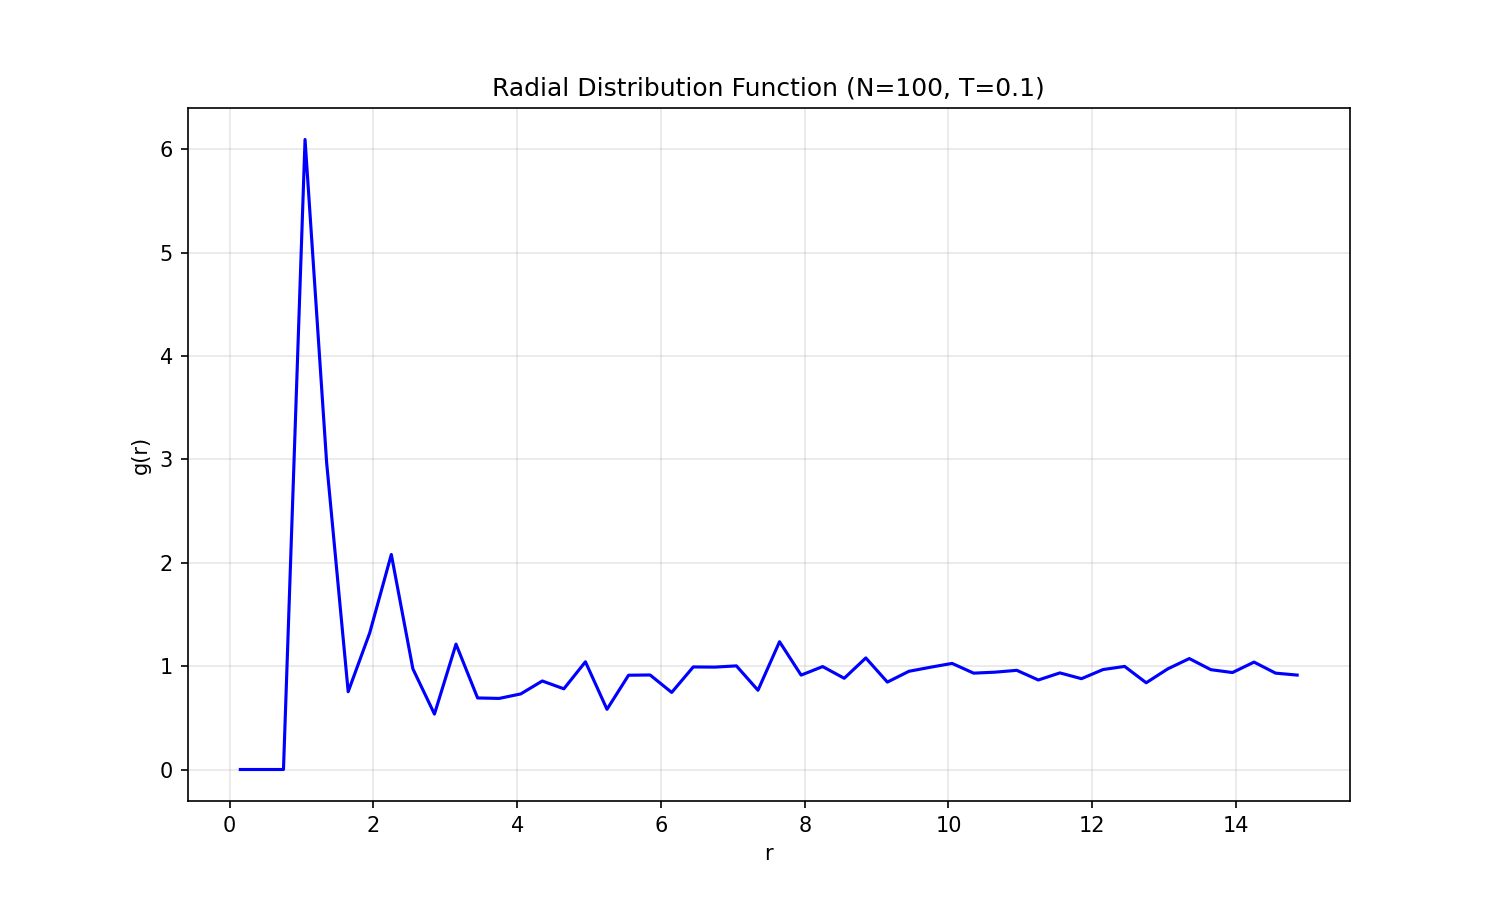
\includegraphics[width=\textwidth]{media/rdf_N100_T0.1.png}
		\caption{N=100 particles with T=0.1}
		\label{sfig:nvt_rdf_N100_T01}
	\end{subfigure}%
	~
	\begin{subfigure}{0.5\textwidth}
		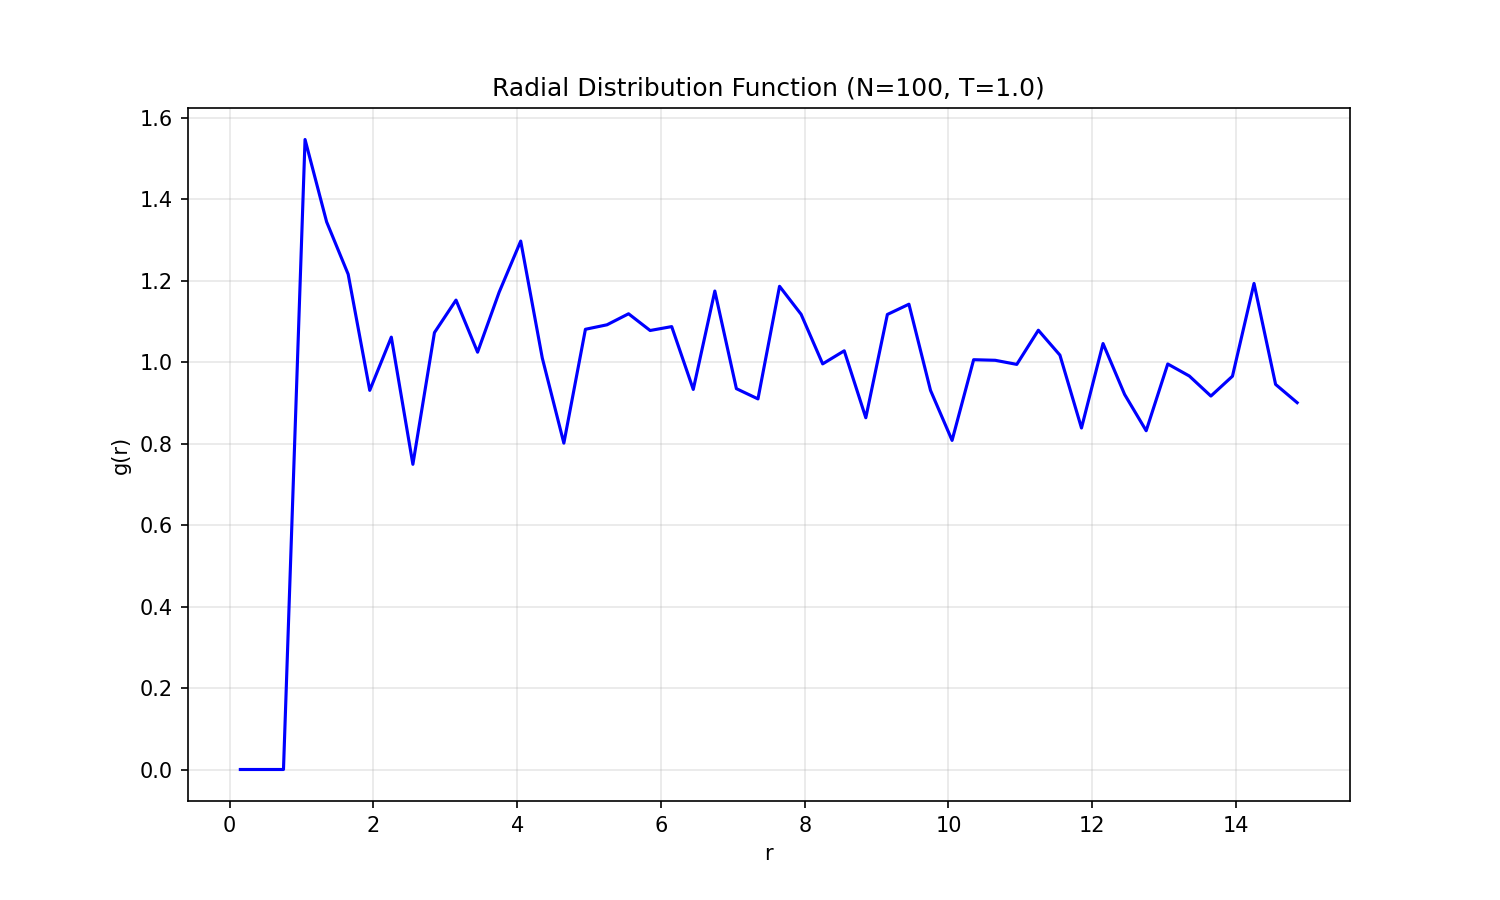
\includegraphics[width=\textwidth]{media/rdf_N100_T1.0.png}
		\caption{N=100 particles with T=1.0}
		\label{sfig:nvt_rdf_N100_T10}
	\end{subfigure}%
	\\
	\begin{subfigure}{0.5\textwidth}
		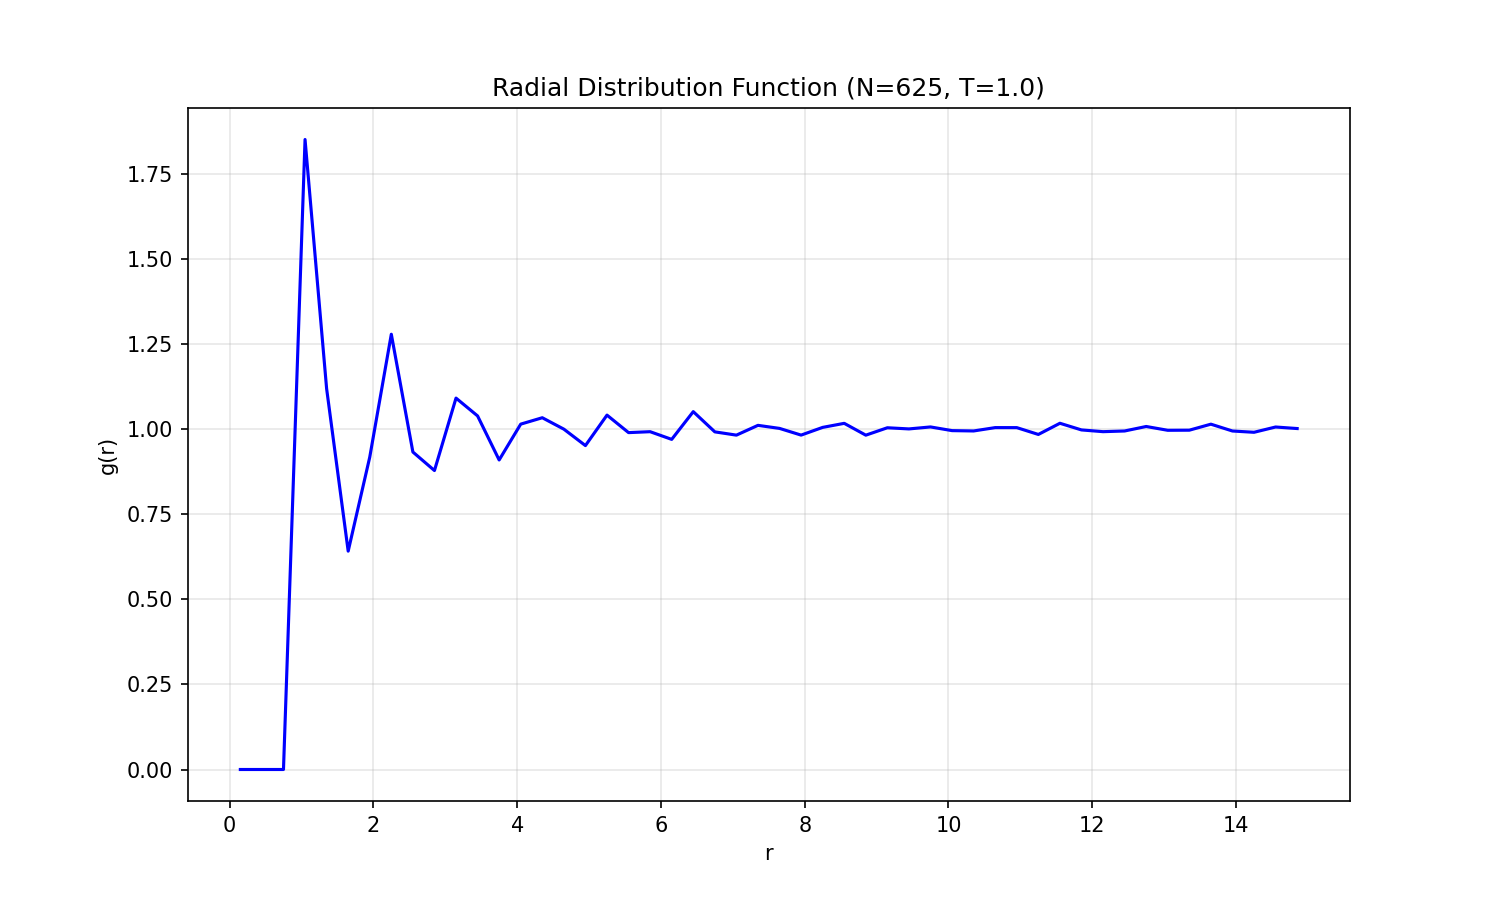
\includegraphics[width=\textwidth]{media/rdf_N625_T1.0.png}
		\caption{N=625 particles with T=1.0}
		\label{sfig:nvt_rdf_N625_T10}
	\end{subfigure}%
	~
	\begin{subfigure}{0.5\textwidth}
		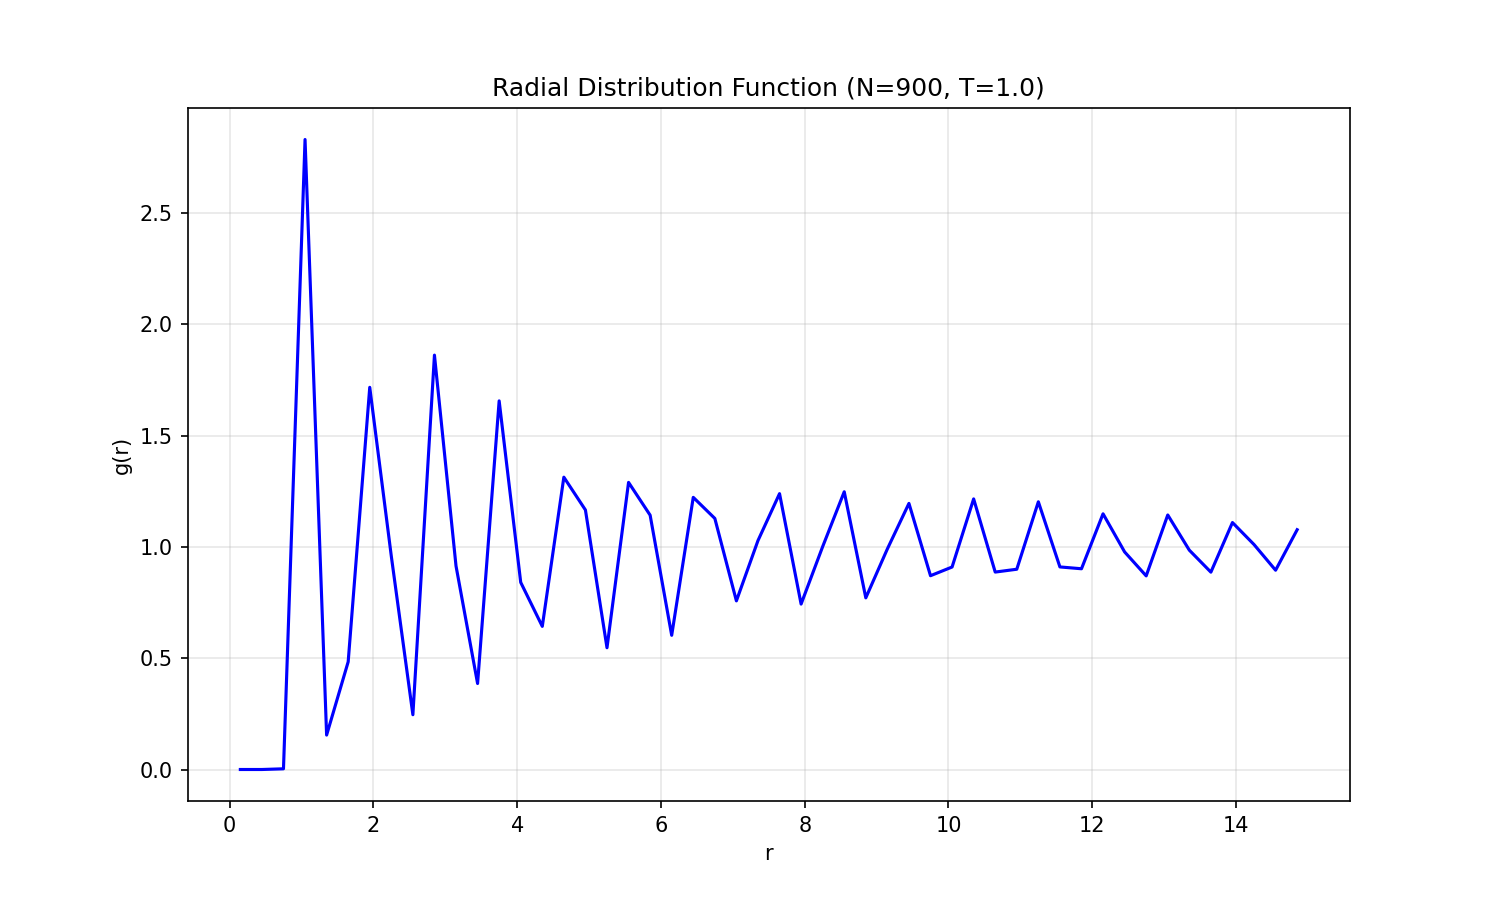
\includegraphics[width=\textwidth]{media/rdf_N900_T1.0.png}
		\caption{N=900 particles with T=1.0}
		\label{sfig:nvt_rdf_N900_T10}
	\end{subfigure}%
	\caption{\textbf{Radial Distribution Functions in NVT Ensemble}
		Radial distribution functions for different system configurations}
	\label{fig:nvt_rdf}
\end{figure}

\section*{Conclusion}
This study showed that the Lennard-Jones systems in NVE and NVT ensemble revealed multiple key findings. The NVE simulations with energy conservation was strongly depending on the step size with smaller steps yielding a better conservation.
Furthermore the systems with a larger number of particles show greater stability and faster equilibration.\\
\\
In NVT simulation, the Berendsen thermostat effectively regulated the temperature with different degrees of precision depending on the system configuration. The phase showed different behaviour depending on the number of particles and target temperature. Furthermore the RDF provided a very valuable insight to determine these states, with the peaks serving as sort of fingerprint to identify the state.


\section{Poiseuille flow with ring-molecules}
For the Poiseuille flow simulation, two stationary walls were placed on opposite sides of the domain, and a constant body force $F_{body} = 0.3$ was applied to all non-wall particles. The system contained $10$ ring molecules (each with 9 particles of type A) alongside fluid particles. Bond parameters were $K_S = 100$ and $r_S = 0.3$.

\subsection{Flow Profile Analysis}
The velocity profile in Figure \ref{fig:poiseuille} shows the characteristic parabolic shape expected for Poiseuille flow, with maximum velocity in the center of the channel and zero velocity at the walls. This confirms the correct implementation of the body force and wall boundary conditions.

\subsection{Molecule Distribution and Evolution}
The ring molecules show a distinct distribution pattern across the channel:
\begin{enumerate}
	\item Initially randomly distributed, the rings gradually migrate toward the center of the channel over time.
	\item The molecule distribution histogram shows higher concentrations near the center and decreased presence near the walls.
	\item The rings appear to maintain their circular structure throughout the simulation, showing the effectiveness of the bond implementation.
\end{enumerate}

The migration of ring molecules toward the center is a phenomenon known as "cross-stream migration" or "tubular pinch effect." This effect has been observed in both simulations and experiments of flowing suspensions. The primary reason for this migration is the balance between:
\begin{enumerate}
	\item Wall-induced migration: The interaction with walls creates an effective repulsive force pushing particles away from the walls.
	\item Shear-induced migration: The non-uniform shear rate across the channel (highest near walls, lowest at center in Poiseuille flow) creates a driving force that moves particles from high-shear to low-shear regions.
\end{enumerate}
This effect is particularly pronounced for extended structures like our ring molecules, as they experience different shear forces across their structure when oriented obliquely to the flow. The resulting hydrodynamic lift pushes them toward the center of the channel where the shear rate is minimal.
Literature on the subject (e.g., Fedosov et al., "Cross-stream migration of deformable particles in microfluidic channels") confirms this behavior for various particle shapes in pressure-driven flows.

\begin{figure}[H]
	\begin{center}
		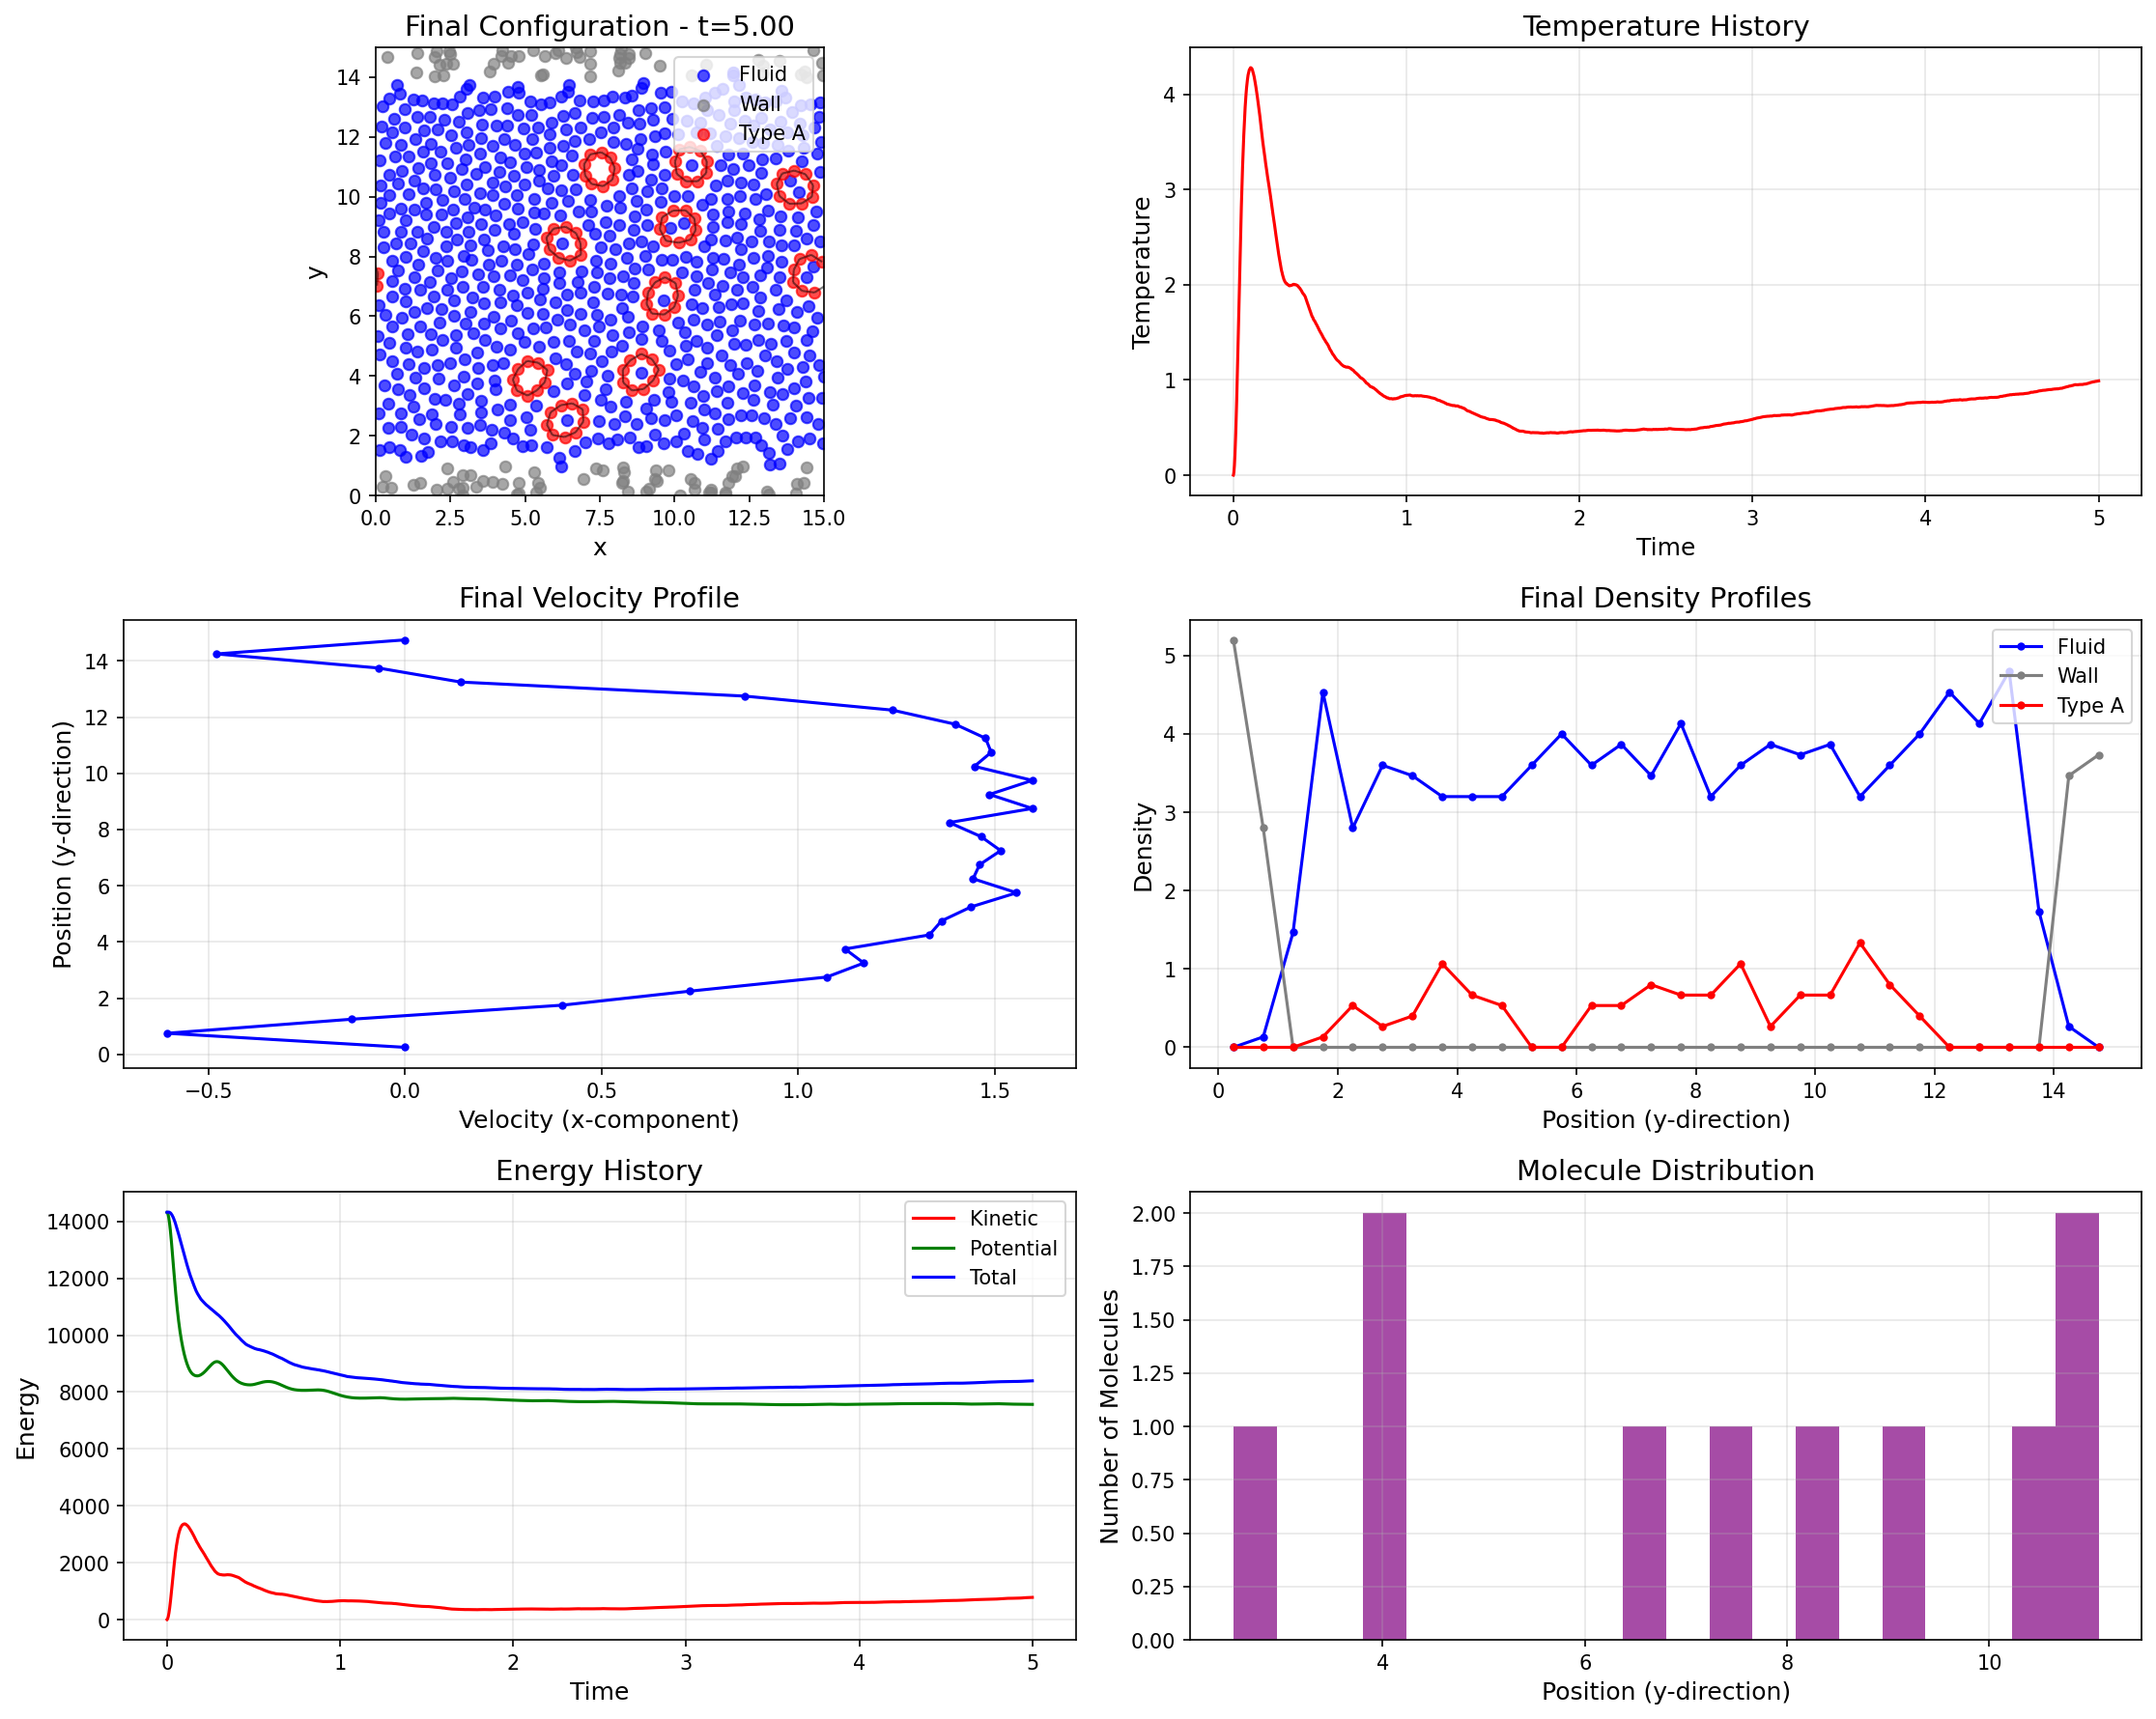
\includegraphics[width=0.95\textwidth]{figures/poiseuille_vis_final.png}
	\end{center}
	\caption{Poiseuille flow with $dt=0.001$ with $5000$ steps}\label{fig:poiseuille}
\end{figure}

\section*{Conclusion}
The DPD simulations successfully captured the expected behaviors of both Couette and Poiseuille flows. The implementation of chain and ring molecules demonstrated the capability of DPD to model complex fluids with structured components.
Key findings include:
\begin{enumerate}
	\item The DPD thermostat effectively maintained system temperature around the desired value.
	\item Chain molecules in Couette flow aligned with the flow direction and showed some level of aggregation.
	\item Ring molecules in Poiseuille flow exhibited cross-stream migration toward the center of the channel, consistent with theoretical predictions and experimental observations.
\end{enumerate}
These simulations illustrate the power of DPD as a mesoscopic simulation method that can capture complex phenomena at the interface between molecular and continuum scales. The soft repulsive potentials and momentum-conserving thermostat make it particularly suitable for simulating soft matter and complex fluids.


\end{document}
